% ATLAS research monograph — main file.
% Build: latexmk -pdf main.tex   (from memoire/). Tables in tables/ and figures in figures/ are GENERATED
% from reports/tables/ by scripts/26_tables_memoire.py and scripts/20_figures_rapport.py: do not edit by hand.
\documentclass[11pt,a4paper]{article}

\usepackage[T1]{fontenc}
\usepackage[utf8]{inputenc}
\usepackage[english]{babel}
\usepackage{mathpazo}
\usepackage{tgpagella}
\usepackage[scaled=0.92]{helvet}
\renewcommand{\ttdefault}{lmtt}
\usepackage{microtype}
\usepackage[margin=2.6cm]{geometry}
\usepackage{setspace}
\setstretch{1.12}
\usepackage{amsmath,amssymb,bm}
\usepackage{graphicx}
\usepackage{booktabs,threeparttable,array,longtable}
\usepackage[font=small,labelfont=bf]{caption}
\usepackage{float}
\usepackage{enumitem}
\setlist{itemsep=2pt,topsep=4pt}
\usepackage{siunitx}
\sisetup{group-separator={,},output-decimal-marker={.}}
\usepackage[dvipsnames]{xcolor}
\usepackage{csquotes}
\usepackage[backend=biber,style=authoryear,maxcitenames=2,maxbibnames=6,uniquelist=false,dashed=false,useprefix=true,doi=true,url=false,isbn=false,eprint=false]{biblatex}
\addbibresource{references.bib}
\usepackage[colorlinks=true,linkcolor=MidnightBlue,citecolor=MidnightBlue,urlcolor=MidnightBlue]{hyperref}
\hypersetup{
  pdftitle={Summer Heat, Irrigation and Crop Yields in France: Pre-specified Estimates and the Empirical Size of Tests in Panels with Common Shocks},
  pdfauthor={Maxime Gourguechon},
  pdfsubject={Working paper (not peer reviewed)},
  pdfkeywords={heat stress; irrigation; maize; France; panel data; wild cluster bootstrap; pre-specification}
}
\usepackage[capitalise,noabbrev]{cleveref}

% GÉNÉRÉ par scripts/26_tables_memoire.py à partir de reports/tables/ : ne pas modifier à la main.
\newcommand{\QoneBeta}{0.0158}
\newcommand{\QonePct}{1.6}
\newcommand{\QoneP}{0.007}
\newcommand{\QoneN}{435}
\newcommand{\QoneReplPct}{1.1}
\newcommand{\QoneReplP}{0.049}
\newcommand{\PowerCheckSize}{5.3}
\newcommand{\PowerHalf}{24}
\newcommand{\PowerFull}{66}
\newcommand{\ReplSize}{5.7}
\newcommand{\ReplPower}{11}
\newcommand{\CiNinetyLow}{0.55}
\newcommand{\CiNinetyHigh}{4.5}
\newcommand{\CiNinetyFiveLow}{0.45}
\newcommand{\CiNinetyFiveHigh}{5.0}
\newcommand{\WheatCiLow}{-7.6}
\newcommand{\WheatCiHigh}{2.4}
\newcommand{\LooMinPct}{1.2}
\newcommand{\LooMaxPct}{1.9}
\newcommand{\LooSig}{17}
\newcommand{\NoReliefPct}{1.0}
\newcommand{\NoReliefP}{0.146}
\newcommand{\NoSwiPct}{1.7}
\newcommand{\NoSwiP}{0.001}
\newcommand{\PetPct}{1.2}
\newcommand{\PetP}{0.035}
\newcommand{\CorrPet}{-0.47}
\newcommand{\DecDiff}{-0.0113}
\newcommand{\DecDiffP}{0.50}
\newcommand{\DecDiffNoThree}{0.0106}
\newcommand{\DecDiffNoThreeP}{0.77}
\newcommand{\EobsPct}{1.5}
\newcommand{\EobsP}{0.005}
\newcommand{\EobsCorr}{0.95}
\newcommand{\RelInter}{0.0087}
\newcommand{\RelInterP}{0.777}
\newcommand{\IrrInterP}{0.415}
\newcommand{\SilageShare}{28}
\newcommand{\SilageP}{0.434}
\newcommand{\DmlBeta}{0.0155}
\newcommand{\DmlP}{0.016}
\newcommand{\CvThreeP}{0.074}
\newcommand{\RiP}{0.001}
\newcommand{\WithinYearSize}{3.7}
\newcommand{\HtwobSize}{4.0}
\newcommand{\HtwocSize}{2.3}
\newcommand{\ConleyFixedPct}{24}
\newcommand{\LevThree}{41}
\newcommand{\LevThreeEarly}{80}
\newcommand{\NeffLevAll}{4.8}
\newcommand{\NeffLevEarly}{1.5}
\newcommand{\EbTau}{0.0045}
\newcommand{\EbQp}{0.199}
\newcommand{\EbMin}{0.012}
\newcommand{\EbMax}{0.021}
\newcommand{\EbCorIrr}{-0.44}
\newcommand{\EbCorAlt}{0.42}
\newcommand{\ForestP}{0.988}
\newcommand{\WindIrrPct}{-0.59}
\newcommand{\WindIrrP}{0.026}
\newcommand{\WindMinP}{0.281}
\newcommand{\ConfCovMin}{95}
\newcommand{\ConfCovMax}{100}
\newcommand{\BzeroTreeMin}{11}
\newcommand{\BzeroTreeMax}{18}
\newcommand{\BzeroTreeSig}{3}
\newcommand{\FodderBeta}{0.0160}
\newcommand{\FodderPct}{1.6}
\newcommand{\FodderP}{0.006}
\newcommand{\FodderSize}{3.0}
\newcommand{\FodderDeps}{28}
\newcommand{\FodderN}{448}
\newcommand{\FodderGap}{35}
\newcommand{\FodderSOnePct}{4.0}
\newcommand{\FodderSOneP}{0.083}
\newcommand{\JunePct}{4.7}
\newcommand{\JuneP}{0.127}
\newcommand{\JaCalPct}{1.3}
\newcommand{\JaCalP}{0.026}
\newcommand{\SeptP}{0.449}
\newcommand{\SeptMean}{0.04}
\newcommand{\JuneMean}{0.32}
\newcommand{\JaMean}{1.9}
\newcommand{\LeadP}{0.351}
\newcommand{\LagP}{0.168}
\newcommand{\LeadMainPct}{1.6}
\newcommand{\IvEobsBeta}{0.0208}
\newcommand{\IvEobsRatio}{1.3}
\newcommand{\IvEobsF}{65}
\newcommand{\IvEobsRfP}{0.005}
\newcommand{\IvLstBeta}{0.0386}
\newcommand{\IvLstRatio}{2.5}
\newcommand{\IvLstF}{13}
\newcommand{\IvLstRfP}{0.002}
\newcommand{\QuadSqP}{0.126}
\newcommand{\BinLowP}{0.582}
\newcommand{\BinMidPct}{7.9}
\newcommand{\BinMidP}{0.135}
\newcommand{\BinHighP}{0.368}
\newcommand{\QuadPredThree}{0.203}
\newcommand{\LinPredThree}{0.202}
\newcommand{\ObsThree}{0.172}
\newcommand{\CompoundInter}{-0.109}
\newcommand{\CompoundP}{0.197}
\newcommand{\VpdPct}{60}
\newcommand{\VpdP}{0.001}
\newcommand{\VpdJointHeatPct}{-0.2}
\newcommand{\VpdJointHeatP}{0.760}
\newcommand{\VpdJointPct}{64}
\newcommand{\VpdJointP}{0.002}
\newcommand{\VpdCorr}{0.76}
\newcommand{\VpdSd}{0.34}
\newcommand{\VpdSdEffect}{17.5}
\newcommand{\FodderVpdP}{0.012}
\newcommand{\FodderHeatJointP}{0.304}
\newcommand{\FodderVpdJointP}{0.124}
\newcommand{\LoyoYearMinPct}{1.4}
\newcommand{\LoyoYearMaxPct}{2.5}
\newcommand{\LoyoYearSig}{26}
\newcommand{\LoyoYearN}{26}
\newcommand{\SerialSizeZero}{6.3}
\newcommand{\SerialSizeLow}{3.7}
\newcommand{\SerialSizeHigh}{9.3}
\newcommand{\MultiN}{76}
\newcommand{\MultiPos}{76}
\newcommand{\MultiSig}{68}
\newcommand{\MultiMedPct}{2.4}
\newcommand{\MultiSurfSig}{24}
\newcommand{\MultiSurfN}{32}
\newcommand{\RuMin}{87}
\newcommand{\RuMax}{134}
\newcommand{\RuInterP}{0.649}
\newcommand{\RuInterBothP}{0.535}
\newcommand{\RuInterAllP}{0.412}
\newcommand{\RuVpdP}{0.006}
\newcommand{\RuCorIrr}{-0.29}
\newcommand{\RuVpdLow}{66}
\newcommand{\RuVpdHigh}{47}
\newcommand{\VolHeatPct}{0.4}
\newcommand{\VolHeatP}{0.284}
\newcommand{\VolVpdP}{0.114}
\newcommand{\VolSwiP}{0.001}
\newcommand{\VolSwi}{-1.60}
\newcommand{\VolN}{202}
\newcommand{\WatDose}{1\,524}
\newcommand{\WatGain}{32}
\newcommand{\WatKg}{2.2}
\newcommand{\WatEur}{0.55}
\newcommand{\WatEurTen}{0.46}
\newcommand{\WatEurMin}{0.17}
\newcommand{\WatEurMax}{0.96}
\newcommand{\WatExcl}{8}
\newcommand{\WatN}{72}
\newcommand{\WatDoseSlope}{74}
\newcommand{\WatDoseSlopeP}{0.039}
\newcommand{\WatGainSlope}{0.36}
\newcommand{\WatGainSlopeP}{0.860}
\newcommand{\DriasModels}{17}
\newcommand{\DriasCtlSim}{1.02}
\newcommand{\DriasCtlMin}{1.00}
\newcommand{\DriasCtlMax}{1.51}
\newcommand{\DriasObsMean}{1.9}
\newcommand{\DriasDdRef}{1.3}
\newcommand{\DriasDdRefMin}{1.0}
\newcommand{\DriasDdRefMax}{1.5}
\newcommand{\DriasDdTwo}{3.8}
\newcommand{\DriasDdTwoMin}{0.8}
\newcommand{\DriasDdTwoMax}{10.5}
\newcommand{\DriasGapTwo}{4}
\newcommand{\DriasGapTwoLow}{1}
\newcommand{\DriasGapTwoHigh}{12}
\newcommand{\DriasVpdTwo}{0.25}
\newcommand{\DriasDdTwoSeven}{7.2}
\newcommand{\DriasDdTwoSevenMin}{1.5}
\newcommand{\DriasDdTwoSevenMax}{12.1}
\newcommand{\DriasGapTwoSeven}{10}
\newcommand{\DriasGapTwoSevenLow}{3}
\newcommand{\DriasGapTwoSevenHigh}{29}
\newcommand{\DriasVpdTwoSeven}{0.42}
\newcommand{\DriasDdFour}{17.9}
\newcommand{\DriasDdFourMin}{8.9}
\newcommand{\DriasDdFourMax}{31.0}
\newcommand{\DriasGapFour}{30}
\newcommand{\DriasGapFourLow}{9}
\newcommand{\DriasGapFourHigh}{106}
\newcommand{\DriasVpdFour}{0.78}
\newcommand{\DriasObsThree}{14.7}
\newcommand{\LstCorr}{0.63}
\newcommand{\LstPct}{4.2}
\newcommand{\LstP}{0.002}
\newcommand{\LstSlope}{0.21}
\newcommand{\LstInterP}{0.051}
\newcommand{\LstSlopeQone}{0.23}
\newcommand{\LstSlopeQthree}{0.19}
\newcommand{\EobsSdEffect}{7.5}
\newcommand{\SimSdEffect}{5.9}
\newcommand{\QoneReplPtwo}{0.10}
\newcommand{\QoneRainfedPct}{2.5}
\newcommand{\QoneIrrigatedPct}{1.0}
\newcommand{\QoneRatio}{2.6}
\newcommand{\QoneHtwoaP}{0.024}
\newcommand{\QoneHtwobP}{<0.001}
\newcommand{\QoneHtwocP}{0.005}
\newcommand{\QoneHthreeP}{0.961}
\newcommand{\QoneSizeWCR}{3.7}
\newcommand{\QoneSizeDep}{16.3}
\newcommand{\QoneSizeConley}{22.0}
\newcommand{\QoneAreaPct}{1.0}
\newcommand{\QoneAreaP}{0.221}
\newcommand{\QoneMaskPct}{1.5}
\newcommand{\QoneMaskP}{0.007}
\newcommand{\QoneValTwoThousandThree}{49}
\newcommand{\QoneValLow}{16}
\newcommand{\QoneValHigh}{170}
\newcommand{\HeatTwoThousandThree}{14.7}
\newcommand{\HeatSecondYear}{4.0}
\newcommand{\HeatRatio}{3.7}
\newcommand{\ReliefGapMin}{7.5}
\newcommand{\ReliefGapMax}{10.3}
\newcommand{\QtwoPct}{1.1}
\newcommand{\QtwoP}{0.125}
\newcommand{\QtwoN}{5,543}
\newcommand{\QtwoWaldP}{0.49}
\newcommand{\QtwoSizeWCR}{4.3}
\newcommand{\QtwoSizeDep}{26.3}
\newcommand{\QtwoSizeConley}{16.3}
\newcommand{\WheatPct}{1.5}
\newcommand{\WheatPdep}{0.004}
\newcommand{\WheatPwcr}{0.374}
\newcommand{\WheatSizeDep}{56}
\newcommand{\WheatSizeConley}{39}
\newcommand{\WheatSizeWCR}{4}
\newcommand{\WheatPowerWCR}{12}
\newcommand{\ForecastWorstPct}{72}
\newcommand{\ForecastBestPct}{14}
\newcommand{\UsualSizeMin}{16}
\newcommand{\UsualSizeMax}{56}
\newcommand{\MaizeDeps}{38}
\newcommand{\MaizeYears}{26}
\newcommand{\MaizeMainDeps}{17}
\newcommand{\MaizeRemoved}{7}
\newcommand{\MaizePairs}{981}
\newcommand{\MaizeMainPairs}{435}
\newcommand{\SpliceN}{1,674}
\newcommand{\SpliceShare}{95}
\newcommand{\SpliceMedian}{0.0}
\newcommand{\SpliceCorrIrr}{0.98}
\newcommand{\SpliceCorrRain}{0.99}
\newcommand{\MaskCorrGrain}{0.993}
\newcommand{\MaskCorrFodder}{0.04}
\newcommand{\WheatDeps}{85}
\newcommand{\WheatMainDeps}{83}
\newcommand{\WheatMainObs}{1,328}
\newcommand{\WheatIntegerShare}{86.6}
\newcommand{\WheatLongMissing}{18}
\newcommand{\WheatLongMissingLast}{1967}
\newcommand{\HeatSeventySix}{1.16}
\newcommand{\HeatPreTwoThousandOtherMax}{0.16}
\newcommand{\SwiMin}{-0.07}
\newcommand{\SwiMax}{1.95}
\newcommand{\SimCells}{9,892}
\newcommand{\SimCellsFrance}{8,984}
\newcommand{\VigiMissEarlyMin}{13}
\newcommand{\VigiMissEarlyMax}{21}
\newcommand{\VigiMissMidMin}{4}
\newcommand{\VigiMissMidMax}{11}
\newcommand{\SpecFourHash}{2a63ada21156}
\newcommand{\SpecFiveHash}{4c9e77872165}
\newcommand{\SpecSixHash}{843f8531055a}
\newcommand{\SpecFourBisHash}{88e15f6290de}
\newcommand{\ConvTinfLag}{0.38}
\newcommand{\ConvTinfSame}{0.58}
\newcommand{\ConvTinfLead}{-0.23}
\newcommand{\ConvTsupLag}{-0.15}
\newcommand{\ConvTsupSame}{0.82}
\newcommand{\ConvTsupLead}{0.08}
\newcommand{\NeffWheat}{4.1}
\newcommand{\NeffWheatNoTwentyFive}{2.64}
\newcommand{\NeffWheatExact}{4.13}
\newcommand{\NeffWheatLong}{6.2}
\newcommand{\NeffMaize}{7.1}
\newcommand{\NeffMaizeShareTwoThousandThree}{26}
\newcommand{\ReliefAltCorr}{-0.93}
\newcommand{\ReliefAltDiffMin}{178}
\newcommand{\ReliefAltDiffMax}{505}
\newcommand{\ReliefCount}{six}
\newcommand{\ReliefCountLarge}{four}
\newcommand{\ReliefGapSmallMin}{4}
\newcommand{\ReliefRhoneMaskGap}{2.8}
\newcommand{\ReliefYonneGap}{2.7}
\newcommand{\SizeDepMin}{16}
\newcommand{\SizeDepMax}{56}
\newcommand{\SizeConleyMin}{16}
\newcommand{\SizeConleyMax}{39}
\newcommand{\SizeWcrMin}{3.5}
\newcommand{\SizeWcrMaxButOne}{4.3}
\newcommand{\SizeWcrMax}{7.0}
\newcommand{\WheatPowerWCRDouble}{29}
\newcommand{\SimR}{300}
\newcommand{\ExRegion}{19.7}
\newcommand{\ExCrOne}{5.0}
\newcommand{\ExWcr}{4.0}
\newcommand{\QoneSwi}{-0.35}
\newcommand{\QoneHthreeEst}{0.0008}
\newcommand{\QoneHthreeN}{168}
\newcommand{\QoneHthreePright}{0.039}
\newcommand{\QoneRobN}{10}
\newcommand{\QoneRobSig}{9}
\newcommand{\QoneRobPos}{10}
\newcommand{\QoneRecentPct}{2.5}
\newcommand{\QoneAllDepsPct}{2.2}
\newcommand{\AreaEarly}{-0.0009}
\newcommand{\MaskEarly}{0.0108}
\newcommand{\AreaRecent}{0.0381}
\newcommand{\MaskRecent}{0.0242}
\newcommand{\CompEst}{-0.0025}
\newcommand{\CompP}{0.58}
\newcommand{\ValAltPct}{29}
\newcommand{\ArMaize}{0.08}
\newcommand{\ArWheat}{0.13}
\newcommand{\GapObsTwoThousandThree}{0.172}
\newcommand{\GapPredTwoThousandThree}{0.202}
\newcommand{\ValOverPct}{17}
\newcommand{\MainShareArea}{36}
\newcommand{\IrrShareOfRainfedSens}{38}
\newcommand{\YieldIrr}{108}
\newcommand{\YieldRain}{77}
\newcommand{\GapMedianPct}{38}
\newcommand{\GapNotAboveCount}{4}
\newcommand{\GapBelowCount}{1}
\newcommand{\ExploPairs}{270}
\newcommand{\ExploSharePct}{62}
\newcommand{\WheatHtwoPwcr}{0.32}
\newcommand{\WheatHtwoPdep}{<0.001}
\newcommand{\WheatRobPreTot}{9}
\newcommand{\WheatRobPreNeg}{8}
\newcommand{\WheatRobAddTot}{3}
\newcommand{\WheatRobAddNeg}{3}
\newcommand{\WheatNoTwentyFivePct}{2.9}
\newcommand{\LoyoNeg}{16}
\newcommand{\LoyoTot}{16}
\newcommand{\QtwoRobNeg}{5}
\newcommand{\QtwoRobTot}{5}
\newcommand{\QtwoRobSig}{1}
\newcommand{\QtwoNoTwentyFiveP}{0.028}
\newcommand{\QtwoNoTwentyFivePtwo}{0.056}
\newcommand{\SlopeA}{0.1}
\newcommand{\SlopeB}{2.8}
\newcommand{\SlopeC}{1.1}
\newcommand{\RfVsBoneSkill}{16}
\newcommand{\BzeroBeatsBone}{10}
\newcommand{\NdviGainMin}{1.6}
\newcommand{\NdviGainMax}{27.7}
\newcommand{\NdviSig}{4}
\newcommand{\NdviTot}{6}
\newcommand{\NdviBeatsBzero}{0}
\newcommand{\VerR}{4.5.2}
\newcommand{\VerFixest}{0.14.2}
\newcommand{\VerRepoDate}{2026-09-26}
\newcommand{\VerPandas}{3.0.6}
\newcommand{\VerSklearn}{1.9.1}
\newcommand{\VerDuckdb}{1.5.5}
\newcommand{\VerGeopandas}{1.1.4}
\newcommand{\VerUvDate}{2026-09-26}
\newcommand{\TestCount}{1127}
\newcommand{\TestIntegrity}{1006}
\newcommand{\TestLogic}{121}
\newcommand{\ManifestFiles}{1,006}
\newcommand{\DdCases}{500}
\newcommand{\DdMaxErr}{8.9 \times 10^{-10}}
\newcommand{\DdDoubleSame}{yes}

\newcommand{\ddthirtytwo}{\ensuremath{\mathrm{DD}_{>32}}}
\newcommand{\degreeday}{\,$^{\circ}$C$\cdot$day}

\title{Summer Heat, Irrigation and Crop Yields in France:\\
Pre-specified Estimates and the Empirical Size of Tests in Panels with Common Shocks}
\author{Maxime Gourguechon}
% Dépôt public et DOI Zenodo du code (DOI de concept, toutes versions de l'archive).
\newcommand{\RepoLink}{\url{https://github.com/maxime2476/Atlas}, archived as \href{https://doi.org/10.5281/zenodo.23305095}{doi:10.5281/zenodo.23305095}}
\date{October 2026 \\ \small Working paper --- not peer reviewed. Code and data pipeline: \RepoLink. \\ \small Text licensed under CC BY 4.0; code under the MIT licence.}

\begin{document}
\maketitle
\begin{abstract}
\noindent Does the yield advantage of irrigated maize grow with extreme summer heat? French agricultural statistics report grain maize yields \emph{separately} for irrigated and rainfed land, by department. I relate the gap between the two, 2000--2025, to degree-days above 32\,$^{\circ}$C in July--August measured on the parcels where maize grows. The specification was written after an exploratory analysis of 2010--2025 and before any estimate on 2000--2009. In 17 departments outside the South-West (\QoneN{} department-years), each degree-day is associated with a \QonePct\,\% higher ratio of irrigated to rainfed yield, so that the median advantage of \GapMedianPct\,\% would become \GapMedianAfterPct\,\% (one-sided wild cluster bootstrap by year, $p = \QoneP$; measured size \QoneSizeWCR\,\%; 90\,\% interval \CiNinetyLow{} to \CiNinetyHigh\,\%). This meets the pre-specified rule, with four reservations. \ExploSharePct\,\% of the sample comes from the exploratory years, and the new decade keeps the sign at about half the estimate ($p = \QoneReplP$). Without the six departments with uplands the result is not significant; a cluster-jackknife statistic is not significant against a Student distribution ($p = \CvThreeP$) but is when bootstrapped ($p = \CvBootP$, size \CvBootSize\,\%). In the older release of the statistics, the irrigated-to-rainfed ratio repeats from one year to the next more often than chance, as an imputation would make it, and a pre-declared check classes this as a live threat. And with the vapour pressure deficit in the model, the association moves to the drying power of the air: it concerns hot, dry summers rather than heat alone. It holds with station-based temperatures and with satellite surface temperature, replicates on silage maize, and all \MultiN{} specifications of a multiverse analysis give a positive estimate; early, coarse estimates for the hot summer of 2026 point the same way. A pre-specified interaction with water restrictions has the opposite sign to the hypothesis. The result is an association, not the causal effect of irrigation. A methodological check changed the conclusions: standard errors clustered by department, or Conley, reject a true null in \UsualSizeMin\,\% to \UsualSizeMax\,\% of placebo simulations on these panels, and with them heat would have appeared ``significantly'' associated with lower wheat yields ($p = \WheatPdep$, against $p = \WheatPwcr$ with a correctly sized test). Wheat yields over 1959--2025 and out-of-sample forecasts give null results, reported in full.

\medskip\noindent\textbf{Keywords:} heat stress; irrigation; maize; France; panel data; wild cluster bootstrap; pre-specification.\\
\textbf{JEL codes:} Q15, Q54, C23, C12.
\end{abstract}

\tableofcontents
\clearpage

\section{Introduction}
\label{sec:introduction}

In the maize departments studied here, July and August 2003 brought \HeatTwoThousandThree{} degree-days above 32\,$^{\circ}$C on average, \HeatRatio{} times more than any other summer since 2000 (\cref{fig:projections}). Maize suffered, but not all maize equally: in the same department, fields with irrigation and fields without it did not lose the same share of their harvest. This monograph asks how large that difference is, how it moves with heat, and how sure we can be about it.

The question matters because irrigation is expensive and because its water is scarcest exactly when it is most valuable. In hot, dry summers, French prefectures issue orders that restrict water withdrawals and can limit irrigation (\cref{sec:data}). Knowing how the yield advantage of irrigated maize varies with summer heat is a first step towards valuing that water.

\subsection*{What we already know}

Extreme heat lowers the yields of the major field crops, in France as elsewhere \parencite{schlenker2009,gammans2017}. Studies abroad find that irrigation weakens this association. In the United States, yield declines on hot days are much weaker in irrigated areas than under rainfed conditions \parencite{schauberger2017}, and the benefit of irrigation depends on growing-season climate \parencite{li2018}. In India, irrigated wheat shows about a quarter of the heat sensitivity of rainfed wheat \parencite{zaveri2019}. Field trials in Kansas point the same way \parencite{tack2017}.

For France, the evidence is indirect. \textcite{hawkins2013} infer a role for irrigation from the declining sensitivity of maize yields to rainfall. \textcite{vandervelde2010} simulate irrigated and rainfed maize with a crop model during the 2003 heatwave and weight the simulations by regional irrigated shares. I am not aware of a statistical estimate built on observed irrigated and rainfed yields.

\subsection*{What this monograph does}

\paragraph{It compares irrigated and rainfed maize side by side.} The French annual agricultural statistics (\emph{Statistique agricole annuelle}) report grain maize yields separately for irrigated and rainfed land in each department. I located an older release that extends this split back to 2000 and checked it against the current one, which gives 26 harvests. The outcome is the log yield gap between the two modes in the same department and year. Shocks that hit both modes proportionally in a given year, for instance a disease outbreak or a late frost if it hits both modes alike, cancel out in the gap. Stable differences between irrigated and rainfed land, such as soils or farm types, are absorbed by department effects. What is left is how the advantage of irrigated maize moves with summer heat.

\paragraph{It measures heat where the maize grows.} Degree-days above 32\,$^{\circ}$C are computed for each 8~km grid cell and each day, then averaged over each department with weights given by the area of maize parcels. The choice matters. In the \ReliefCount{} departments with uplands, a department-wide average understates the heat that maize experienced in July--August 2003 by \ReliefGapSmallMin{} to \ReliefGapMax{} degree-days (\cref{tab:relief}; \cref{fig:map} shows where they lie), and with that measure the main result is no longer significant (\cref{sec:maize}).

\paragraph{It checks whether its own tests can be trusted.} This is where the project took its most important turn. For wheat, heat at the end of the cycle was associated with \WheatPct\,\% lower yields per degree-day. Two of the three inferences planned in advance called this significant: $p = \WheatPdep$ with standard errors clustered by department. The third, a bootstrap by year, did not ($p = \WheatPwcr$). Which one to believe? I asked a simple question: if heat had no effect at all, how often would each test still say it does? To find out, I replaced each year's heat with the heat of another year, keeping its real geography, and re-ran the tests hundreds of times. Clustering by department said ``significant'' \WheatSizeDep\,\% of the time, instead of the nominal 5\,\%. A hot summer is hot everywhere, so 83 departments are not 83 independent experiments, and the usual standard errors behave as if they were.

The problem is not specific to wheat or to this project. Across the five size checks run here, on three panels (\cref{tab:sizes}), standard errors clustered by department and \textcite{conley1999} standard errors with a 200~km cut-off (uniform kernel, no serial component, as implemented here) reject a true null in \UsualSizeMin\,\% to \UsualSizeMax\,\% of cases. A wild cluster bootstrap with clusters by year and Webb weights \parencite{cameron2008,webb2023} stays close to 5\,\%, and it is the only inference on which the conclusions below rely. This size check was not in the original plan; it was added as a diagnostic, and it is now applied to every main test. \Cref{sec:inference} explains the check so that others can run it on their own data; the code is a stand-alone module (\cref{app:wcr}).

\paragraph{It fixed its rules in advance, and says where it did not.} Each estimation phase began with a written specification whose SHA-256 hash was recorded in the project's decision log before any estimate of that phase was computed. The log is published with the code, but it was kept by the author alone, and the specifications, the log and the results are published together. The hashes therefore show only that the files have not changed since publication; that each specification came before its estimates, and that each check added later was declared before it was computed, is the author's statement. For maize, the decision rule was set at the same time: a hypothesis counts as established only if its one-sided bootstrap $p$-value is below 0.05 \emph{and} the measured size of the test is at most 10\,\%. The maize specification was not written blind, since an exploratory analysis of 2010--2025 already existed; this is why the untouched years 2000--2009 serve as a replication. Some analyses were added after results were known: the size checks themselves, extra robustness checks for wheat, and the comparison of the forecasts with the department mean (B0), a benchmark defined in the specification but not used as its criterion. They are reported as such, and every departure from the plans is listed in \cref{app:deviations}.

\subsection*{What I find}

In the 17 departments with the best quality status (the 2025 status, applied to the whole period), each degree-day above 32\,$^{\circ}$C in July--August is associated with a \QonePct\,\% wider gap in favour of irrigated maize, that is, a \QonePct\,\% higher ratio of irrigated to rainfed yield: at the median, an advantage of \GapMedianPct\,\% would become \GapMedianAfterPct\,\% (\cref{fig:maize-resid}; $p = \QoneP$; the test's measured size is \QoneSizeWCR\,\% and \PowerCheckSize\,\% in two placebo runs). Each degree-day is associated with about \QoneRainfedPct\,\% lower rainfed yields and \QoneIrrigatedPct\,\% lower irrigated yields. On these point estimates, rainfed maize is thus about \QoneRatio{} times more sensitive to heat (the size of these two tests, measured afterwards, is \HtwobSize\,\% and \HtwocSize\,\%).

This meets the rule fixed in advance, but the evidence is weaker than the $p$-value suggests. \ExploSharePct\,\% of the department-years belong to 2010--2025, the period whose exploratory analysis suggested the hypothesis; the only new evidence is the decade 2000--2009. Its magnitude is uncertain: the 90\,\% interval obtained by inverting the bootstrap runs from \CiNinetyLow{} to \CiNinetyHigh\,\% per degree-day. With the maize mask, the estimate is \MaskRecent{} on 2010--2025 and \MaskEarly{} on 2000--2009; the difference comes from 2003, since without that summer the earlier decade gives a larger estimate (\cref{tab:maize-measure}). The exploratory analysis, with department-wide weather, had given \AreaRecent{} on 2010--2025, and that measure gives $\AreaEarly$ on 2000--2009.

Eight checks shape how far this result can be trusted.
\begin{itemize}
  \item \textbf{New years.} On 2000--2009 alone, a decade no earlier analysis had touched, the estimate keeps its sign with the maize mask, at about half the 2010--2025 estimate (\QoneReplPct\,\% against \QoneRecentPct\,\%, one-sided $p = \QoneReplP$; the specification set no threshold for the replication). With department-wide weather it does not.
  \item \textbf{An older map of maize.} With a 2008 map of parcel blocks (grain and silage maize) instead of 2015--2017 parcels, almost nothing changes (\QoneMaskPct\,\%, $p = \QoneMaskP$).
  \item \textbf{Department-wide weather.} With heat averaged over the whole department, the estimate is not significant ($p = \QoneAreaP$). \Cref{sec:maize} shows that this measure understates the 2003 heat where maize grows in departments with uplands, a pattern found after the fact; it does not explain the whole divergence, and why this measure gives a stronger association over 2010--2025 is unexplained.
  \item \textbf{Departments with uplands.} Dropping any single department leaves the estimate significant (\LooMinPct{} to \LooMaxPct\,\%), but without the six departments with uplands it falls to \NoReliefPct\,\% and is not significant ($p = \NoReliefP$). Under the rule declared before this check, the result depends on those departments, where the measure of heat also matters most; but their slope does not differ detectably from that of the others ($p = \RelInterP$), so the other departments may simply carry less information.
  \item \textbf{Another inference.} 2003 carries \LevThree\,\% of the useful variation in heat. With so much weight on one cluster, another valid inference, the cluster jackknife, gives $p = \CvThreeP$ against a Student distribution; bootstrapping the same statistic, as recommended when one cluster carries high leverage, gives $p = \CvBootP$ with a measured size of \CvBootSize\,\% (a check added later). The evidence is therefore weaker under some reasonable tests than under others.
  \item \textbf{Another crop.} Silage maize, whose irrigated and rainfed yields the statistics also report for 2010--2025, shows the same association (\FodderPct\,\% per degree-day, $p = \FodderP$, \FodderDeps{} departments), and the heat of the following summer, which cannot affect the harvest, shows none.
  \item \textbf{Heat or dry air?} When the vapour pressure deficit, the drying power of the air, enters the model with degree-days, it carries the association (\VpdJointPct\,\% per kPa, $p = \VpdJointP$) and the degree-days lose theirs. The two are too correlated to be separated, so the result is best read as concerning hot, dry summers.
  \item \textbf{Another temperature source.} With E-OBS station-based temperatures instead of SIM2, the estimate is \EobsPct\,\% ($p = \EobsP$); with satellite land-surface temperature in place of degree-days, the gap widens by \LstPct\,\% per degree Celsius ($p = \LstP$).
\end{itemize}

A pre-specified interaction with crisis-level water restrictions (2016--2025) has the opposite sign to the hypothesis: the slope of the gap on heat is not smaller where restrictions lasted longer. The other results are null, and they are reported as fully as the positive one. For soft wheat over 1959--2025, heat at the end of the cycle is associated with \QtwoPct\,\% lower yields per degree-day, but this cannot be told apart from zero ($p = \QtwoP$), and I find no sign that wheat has become more or less sensitive to heat since 1959. Out-of-sample forecasts of wheat yields from weather and satellite NDVI, built as pre-specified, are not significantly better than the simplest benchmark, the historical mean of each department.

\subsection*{What this monograph does not claim}

The maize result is an association, not the causal effect of irrigation. Irrigated and rainfed land differ in ways that may themselves interact with heat, and in dry years part of the rainfed crop sown for grain may be harvested as silage (\cref{sec:discussion}; abandoned fields stay in the statistics with a zero yield). The outcome itself is not fully measured: in the older release used for 2000--2009, the irrigated-to-rainfed ratio repeats exactly from one year to the next far more often than chance (\SaaRepOld{} of the \SaaRepTot{} repetitions of the main sample are in that release), which suggests that part of the split was carried over rather than observed (\cref{subsec:discussion-wrong}). The estimates also concern year-to-year weather shocks. They do not translate directly into the effect of a warmer climate, to which farmers would adapt.

\subsection*{Outline}

\Cref{sec:literature} reviews related work. \Cref{sec:data,sec:exposure,sec:strategy} describe the data, the measurement of heat and the empirical strategy. \Cref{sec:inference} is devoted to inference. \Cref{sec:maize,sec:wheat,sec:forecasting} report the results for maize, wheat and forecasting. \Cref{sec:discussion} discusses limitations and \cref{sec:conclusion} concludes. The appendices cover reproduction, variables, deviations from the plans, full robustness tables, the bootstrap module, the validation of the degree-day computation and further checks on maize.

\section{Related literature}
\label{sec:literature}

This monograph sits where four literatures meet: the effect of heat on crop yields, how irrigation changes the response to heat, inference when shocks are shared across space, and yield forecasting. The review below is targeted, not exhaustive. For each strand I say what is known and what remains open for France.

\subsection{Heat and crop yields}

The modern empirical literature starts from a simple observation: yields respond to heat in a strongly non-linear way. Using United States counties, \textcite{schlenker2009} show that yields of maize, soybeans and cotton rise slowly with temperature up to a threshold of about 29 to 32\,$^{\circ}$C, depending on the crop, and fall steeply above it. The same relation appears in time series and in cross-section. This is why the analysis below separates ordinary growing degree-days from degree-days above a high threshold. Revisiting the question with recent reanalysis data, \textcite{hogan2024} conclude that correctly capturing daily extremes matters more than the choice of weather data set. This supports building extremes at the level of the grid cell and the day before aggregating, as done here (\cref{sec:exposure}).

For France, the effect of heat on cereals is established. \textcite{gammans2017} estimate the response of wheat and barley yields to the full distribution of temperatures over 1950--2015, with department fixed effects, regional quadratic trends and spatially corrected standard errors. All yields fall when spring and summer temperatures rise. The authors also name two limits that matter here. Their data contain little exposure above 34\,$^{\circ}$C, and temperature anomalies may stand in for dry spells, which soil-moisture data would be needed to rule out. \textcite{ceglar2016} relate monthly weather to the year-to-year variability of wheat and maize yields department by department and find strong regional heterogeneity; for maize, irrigation masks the rainfall signal in dry years. \textcite{benari2018} study the unforeseen 2016 wheat loss in the main cereal-growing region, and \textcite{noiajunior2025} attribute past and projected wheat losses in the same region to climate and diseases with a random forest.

Two related questions are not the object of this monograph but shape its reading. The first is the role of water, which \cref{subsec:maize-vpd} examines through checks with the vapour pressure deficit and irrigation volumes. For United States maize, \textcite{lobell2013} argue with a crop model that the damage associated with extreme heat runs largely through the water demand of hot, dry air, measured by the vapour pressure deficit, and through the soil water stress it causes. Heat and drought also tend to occur together, and their joint occurrence does more damage than either alone \parencite{haqiqi2021,lesk2022}. \textcite{rigden2020} find that United States maize yields are predicted better by the combination of atmospheric evaporative demand and soil moisture than by temperature and precipitation, and that a projection driven by atmospheric demand alone would indicate about twice the damage. Using irrigated maize, where soil moisture deficits are largely removed, \textcite{carter2016} find no direct negative effect of daytime air temperature on the yields of irrigated contest fields in Nebraska, Kansas and Missouri, which points the same way. In a crop-model ensemble for Europe, \textcite{webber2018} find that drought, not heat, drives the projected losses of grain maize. In United States counties, \textcite{ortizbobea2019} find that water stress matters for historical yields while direct heat dominates projections; for German districts, \textcite{lischeid2022} find soil moisture less relevant than meteorological drivers. The second is adaptation: \textcite{merel2021} examine when panel estimates of short-run weather effects can inform long-run responses. The estimates below are short-run responses to weather shocks, and I do not claim more.

\subsection{Irrigation and heat sensitivity}

Abroad, several studies compare irrigated and rainfed yields more directly.
\begin{itemize}
  \item In the United States, \textcite{schauberger2017} find that each day above 30\,$^{\circ}$C costs rainfed maize up to about 6\,\% of yield, and irrigated maize much less.
  \item County statistics in the United States report yields separately for irrigated and rainfed land, as the French ones do. With them, \textcite{troy2015} find that irrigation reduces the yield response to every climate extreme they examine, including heat; \textcite{li2018} compare the two across counties of the western United States; and \textcite{luan2021} find that irrigation helps most in hot, dry seasons and, for maize, reverses the response to temperature. A master's thesis using the same paired yields argues that temperature predictors absorb part of the effect of water stress in statistical crop models \parencite{hunter2026}. With crop-insurance losses, \textcite{pinto2026} find the residual effect of extreme heat on irrigated maize indistinguishable from zero (a conference paper, not yet peer reviewed).
  \item In India, \textcite{zaveri2019} estimate that irrigated wheat has about a quarter of the heat sensitivity of fully rainfed wheat.
  \item In Kansas field trials, \textcite{tack2017} find that irrigation fully offsets the yield loss that warming causes to dryland wheat in their sample.
  \item Irrigation acts through two channels. With satellite land-surface temperature for Nebraska maize, \textcite{zhu2022} attribute about two thirds of the yield benefit of irrigation to relieved water stress and one third to relieved heat stress, through cooling that air temperature does not show. For Europe, \textcite{siebert2017} show that heat stress computed from air temperature is overestimated on irrigated land. Both points matter here: the heat measure below is air temperature, the same for irrigated and rainfed fields.
\end{itemize}

For France, the evidence is indirect. \textcite{hawkins2013} document the growing influence of heat on French maize yields since the 1960s and infer a role for irrigation from the declining sensitivity of yields to rainfall. \textcite{vandervelde2010} simulate irrigated and rainfed maize with the EPIC crop model during the 2003 heatwave, weight the simulations by regional irrigated shares and check them against reported regional yields, and \textcite{vandervelde2012} evaluate regional crop simulations against observed yields in extreme years. None of these studies compares observed irrigated and rainfed yields within the same department and year. That comparison is the core of this monograph. Its design is not new: it follows the American studies above. What it adds is the French case, the gap within the same unit and year, a heat measure built on the parcels where maize grows, and tests whose size is measured on the data.

\subsection{Inference when shocks are shared}

Weather is a common shock. A hot summer raises temperatures in most departments at once, and it lowers yields in most of them at once. The resulting correlation across units within a year is not removed by year fixed effects, which only remove its average, whenever the intensity of the shock varies across space.

Two standard responses exist. The first is to allow for spatial correlation within a distance cut-off, following \textcite{conley1999}. The second is to cluster by time period. Clustering by period leaves few clusters. \textcite{cameron2008} show that tests based on clustered standard errors can over-reject with few clusters (five to thirty), and that a wild cluster bootstrap-$t$ performs much better. \textcite{webb2023} proposes a six-point weight distribution for the case of very few clusters, and \textcite{mackinnon2017} study how the wild cluster bootstrap behaves when cluster sizes differ widely. This monograph uses the restricted wild cluster bootstrap-$t$ of \textcite{cameron2008}, with years as clusters and the weights of \textcite{webb2023}. \textcite{mackinnon2023} review these methods and also recommend the cluster jackknife (CV3) when a few clusters carry much of the leverage, as 2003 does here; it is reported as a check.

Measuring how often a test rejects a true null with placebo treatments is an established practice: \textcite{bertrand2004} generate placebo laws in state panels and find ``significant'' effects for up to 45\,\% of them, and \textcite{mackinnon2017} also simulate placebo laws. I apply this practice to weather panels, with a placebo that keeps the real spatial structure of each year's exposure, run on the data of each question (\cref{sec:inference}). The answer turns out to decide which conclusions can be drawn.

\subsection{Forecasting yields out of sample}

The forecasting literature warns that validation design drives reported performance.
\begin{itemize}
  \item \textcite{gouache2015} build an operational forecasting tool for French departmental wheat yields. On new years (2011--2014), its errors are about twice as large as in leave-one-year-out cross-validation.
  \item \textcite{paudel2021} stress the absence of information leakage and the comparison with naive benchmarks in large-scale machine-learning forecasts for European regions.
  \item \textcite{morales2023} find that, with a time-ordered split, even a random forest has only a limited advantage over a sensible benchmark.
\end{itemize}
In the wheat studies reviewed above, variables, thresholds or trends are chosen using the years later used for evaluation \parencite{benari2018,noiajunior2025}. \Cref{sec:forecasting} therefore uses a strictly chronological protocol in which everything is estimated within each training window.

\subsection{Where this monograph fits}

\Cref{tab:positioning} summarises the position of this work. Its contribution is a French application of established designs, with particular attention to inference and to measurement. It is not a new method, and on wheat its estimate has the expected sign but cannot be distinguished from zero.

\begin{table}[H]
\centering
\small
\caption{What is known and what this monograph adds}
\label{tab:positioning}
\begin{tabular}{>{\raggedright}p{3.3cm}>{\raggedright}p{5.4cm}>{\raggedright\arraybackslash}p{5.4cm}}
\toprule
Question & Known & Added here \\
\midrule
Heat and French cereal yields & Established for 1950--2015 \parencite{gammans2017} & Wheat 1959--2025: negative but not distinguishable from zero with a correctly sized test \\
Irrigation and heat sensitivity & Direct evidence abroad, from county yields reported by irrigation status (United States); indirect evidence for France & Within-department, within-year comparison of observed irrigated and rainfed maize yields, 2000--2025 \\
Measuring exposure & Cropland weights or no mask; no difference found in the cereal belt \parencite{benari2018} & In departments with uplands, weighting by maize parcels changes the result \\
Inference & Wild cluster bootstrap with few clusters & Size of every main test measured on its own data \\
Forecasting & Validation design matters & Strictly chronological protocol: no model significantly better than the department mean \\
\bottomrule
\end{tabular}
\end{table}

\section{Data}
\label{sec:data}

All data are public. \Cref{tab:sources} lists the sources; this section explains how each one is used, what was checked, and where the known weaknesses lie. Every raw file is stored unmodified with its URL, access date and SHA-256 hash, and an automated test verifies these hashes (\cref{app:reproduction}).

\begin{table}[H]
\centering
\small
\caption{Data sources}
\label{tab:sources}
\begin{tabular}{>{\raggedright}p{4.4cm}>{\raggedright}p{4.3cm}>{\raggedright}p{2.6cm}>{\raggedright\arraybackslash}p{2.6cm}}
\toprule
Source & Variables used & Coverage & Licence \\
\midrule
Agreste, \emph{Statistique agricole annuelle} (SAA), long series & Area, yield, quality status; wheat, irrigated and rainfed grain maize & Departments, 2010--2025 & Free reuse with attribution; Licence Ouverte 2.0 \\
Agreste, SAA ``older series'' (\texttt{SAANR\_DEVELOPPE\_2}) & Irrigated and rainfed grain maize & Departments, 2000--2020 & Free reuse with attribution \\
\textcite{schauberger2021data}, version RAW; data paper \textcite{schauberger2022} & Soft wheat yields & Departments, 1959--2009 & CC BY 4.0 \\
Météo-France, SIM2 (SAFRAN--ISBA) & Daily Tmin, Tmax, precipitation, evapotranspiration, soil wetness index & 8~km grid, Aug.~1958--2025 & Licence Ouverte 2.0 \\
IGN / ASP, parcel register (RPG) v2.0 & Grain maize and soft wheat parcels & Parcels, 2015--2017 & Licence Ouverte 2.0 \\
IGN / ASP, RPG v1.0 (anonymised blocks) & Blocks whose main crop is maize & 4 regions, 2008 & Licence Ouverte 2.0 \\
IGN, ADMIN EXPRESS COG CARTO & Department boundaries & 2026 edition & Licence Ouverte 2.0 \\
IGN, altimetry service (RGE ALTI) & Mean altitude of grid cells & 8~km cells & Licence Ouverte 2.0 \\
Ministry of Ecological Transition, VigiEau & Water-restriction orders and severity levels & Departments, orders from 2010 (used: 2012--2025) & Licence Ouverte 2.0 \\
INSEE, producer price index (IPPAP); Eurostat \texttt{apri\_ap\_crpouta} & Maize and wheat prices & 2000--2025 & INSEE: Licence Ouverte 2.0; Eurostat: reuse with attribution \\
NASA LP DAAC, MOD13Q1 v6.1 \parencite{didan2021} & NDVI, 250~m, 16-day composites & 2010--2025 & CC0 (NASA), citation requested \\
NASA LP DAAC, MOD11A2 v6.1 \parencite{wan2021} & Daytime land-surface temperature, 1~km, 8-day composites (check only) & July--August 2000--2025 & CC0 (NASA), citation requested \\
ECA\&D / Copernicus, E-OBS v33.0e \parencite{cornes2018} & Daily Tmin, Tmax (check of the heat measure only) & 0.1$^{\circ}$ grid, 2000--2025 & Non-commercial research and education; citation required \\
RTE / ODRÉ, register of electricity installations & Onshore wind capacity, commissioning date (one check only) & Installations, snapshot of June 2026 & Licence Ouverte 2.0 \\
\bottomrule
\end{tabular}
\end{table}

\noindent Sources: Agreste, Statistique agricole annuelle; Météo-France, SIM2; IGN (ADMIN EXPRESS, RPG, RGE ALTI); Ministry of Ecological Transition, VigiEau; Insee; Eurostat; NASA LP DAAC; E-OBS; RTE. We acknowledge the E-OBS dataset and the data providers in the ECA\&D project (\url{https://www.ecad.eu}). The licence terms of Agreste, INSEE, Eurostat and NASA were checked on the producers' websites on 11 October 2026, those of E-OBS and RTE on 12 October 2026; access dates and the attribution of each source are listed in the repository (\texttt{NOTICE.md}, \texttt{docs/manifest\_raw.csv}). The Schauberger et al.\ yields were converted from t/ha to q/ha and matched to INSEE department codes.

\subsection{Crop yields}

\paragraph{Maize: two releases of the same statistics.} The current long series of the SAA (2010--2025) report, for each department, the area and yield of grain maize on irrigated and on rainfed land. I found an older release on the Agreste website, a table of ``developed crops'' published as one file per year for 2000--2020, which contains the same split. The older release was not revised after the 2020 agricultural census, while the long series were. Before splicing them, I compared the two over 2010--2020, where they overlap. Over \SpliceN{} department-year-mode pairs, in all departments, \SpliceShare\,\% of yields agree to within 0.5 quintal per hectare, the median difference is \SpliceMedian{} quintal per hectare, and the correlation is \SpliceCorrIrr{} for irrigated and \SpliceCorrRain{} for rainfed maize. The panel uses the older release for 2000--2009 and the long series from 2010 onwards.

\paragraph{Population and main sample.} The population is the set of departments where both irrigated and rainfed grain maize covered at least 1,000~ha on average over 2010--2012: \MaizeDeps{} departments. The threshold is fixed on 2010--2012, inside the estimation period; the areas of those years could themselves reflect their weather, but the rule does not change with the outcome of any later year. The SAA attaches a quality status to each series; the main sample keeps the \MaizeMainDeps{} departments whose irrigated maize series has status~1, the best. This status is only published for recent years, so the 2025 status is applied to the whole period. The other departments are used as a robustness check.

\paragraph{Exclusions.} \MaizeRemoved{} department-year-mode observations have a missing or zero yield and are dropped; they are listed in the project documentation. The maize models compare the two modes, so they use the \MaizePairs{} department-years where both are observed, of which \MaizeMainPairs{} are in the main sample.

\paragraph{Wheat.} For soft wheat (soft winter wheat in the SAA; ``soft wheat'' below), the SAA long series cover 2010--2025. Over 1959--2009, I use the RAW version of the departmental yields compiled by \textcite{schauberger2022}. Their data come from hand-digitised statistics before 1989 and from the former Agreste database afterwards, and I checked their compatibility with the SAA on the 2010--2018 overlap. The population is the \WheatDeps{} departments with at least 1,000~ha of wheat on average over 2010--2012; the main sample keeps the \WheatMainDeps{} with quality status~1, which gives \WheatMainObs{} observations over 2010--2025. In the long panel, \WheatLongMissing{} yields of the main sample are missing, all in 1959--\WheatLongMissingLast; they are dropped, not imputed.

\paragraph{What yields measure.} SAA yields are a synthesis of several sources, and many are rounded: \WheatIntegerShare\,\% of wheat yields over 2010--2025 are whole numbers of quintals per hectare. Rounding adds noise of at most 0.5 quintal, about 1\,\% of yield, to the outcome. Land is attributed to the department of the farm's headquarters, not to the department of the parcel, which creates small mismatches near borders. The 2025 values are provisional.

\subsection{Weather}

SIM2 is Météo-France's reanalysis combining the SAFRAN atmospheric analysis with the ISBA land-surface model. It provides daily minimum and maximum temperature, precipitation, reference evapotranspiration and a soil wetness index (SWI) on a grid of \SimCells{} cells of 8~km, of which \SimCellsFrance{} intersect a metropolitan department; the others lie at sea or abroad. The SWI is dimensionless. The product documentation labels it as a percentage, but its monthly cell means range from $\SwiMin$ to $\SwiMax$; I read it with the usual definition of Météo-France's index, about 0 at the wilting point and about 1 at field capacity, a reading that the documentation does not state explicitly. The series starts on 1~August~1958, which covers the sowing of the 1959 wheat harvest.

Two features of SIM2 matter for the analysis. First, it is a reanalysis: it interpolates observations and may smooth local extremes; E-OBS, interpolated from stations, indeed counts more degree-days above 32\,$^{\circ}$C in the maize departments (\cref{sec:maize}). Second, the documentation does not state to which calendar day the minimum and maximum temperatures refer. I inferred the convention from the data: the minimum is that of the morning of day $J$ and the maximum that of the afternoon of day $J$ (\cref{sec:exposure}).

\subsection{Where crops grow: the parcel register}

The parcel register (\emph{Registre parcellaire graphique}, RPG) maps the fields declared for the Common Agricultural Policy. Version 2.0 (from 2015) gives each parcel its crop. I use the 2015--2017 vintages to build fixed masks: soft winter wheat (code \texttt{BTH}) and maize (code \texttt{MIS}); one later check uses silage maize (code \texttt{MIE}) in the same way.

Does the code \texttt{MIS} cover grain maize, silage maize, or both? I checked against the SAA. Across departments with more than 2,000~ha, the area of \texttt{MIS} parcels has a correlation of \MaskCorrGrain{} with the SAA area of grain maize and of \MaskCorrFodder{} with the area of silage maize, across department-vintages of 2015--2017. \texttt{MIS} therefore tracks grain maize. It does not, however, say whether a parcel is irrigated.

Version 1.0 (2007--2014) only maps anonymised blocks of parcels, each labelled with its main crop group, where the maize group mixes grain and silage. I use the 2008 vintage, for the four regions that contain the main maize sample, to test whether a mask from 2015--2017 is too recent for the 2000s (\cref{sec:maize}).

\subsection{Water restrictions}

VigiEau publishes the orders by which prefectures restrict water use, with their start and end dates, the zones concerned and a severity level: vigilance, alert, reinforced alert, crisis. From these I count, for each department and summer, the days in July--August when at least one zone is at crisis level. The severity level is missing for almost all orders in 2010--2011, which are dropped, and for \VigiMissEarlyMin\,\% to \VigiMissEarlyMax\,\% of orders in 2012--2015, against \VigiMissMidMin\,\% to \VigiMissMidMax\,\% in 2016--2022. Analyses of restrictions therefore use 2016--2025. The indicator is coarse: it does not say what share of the maize area was restricted.

\subsection{Prices and satellite data}

Prices are only used for a descriptive valuation. The INSEE producer price index for maize gives the year-to-year variation. Eurostat gives absolute prices up to 2016. I convert the index into euros per quintal with its ratio to Eurostat over 2012--2016. A stability criterion was fixed in advance (largest deviation of the ratio below 0.002 euro per quintal per index point); it is met. Three sources, added later, serve checks on soils and water in \cref{sec:maize}. The available water capacity of soils, 0--200~cm, comes from an INRAE map at 90~m \parencite[data: doi:10.15454/9IRARJ]{romandobarco2019}; I average it over the pixels whose centre lies in a grain maize parcel of the RPG in 2015, 2016 or 2017. Volumes withdrawn for irrigation come from the national database of water withdrawals (BNPE, via the Hub'Eau API), declared by each withdrawal point and year, for all crops; withdrawals below the fee threshold of the water agencies (10\,000~m$^3$ a year in most areas) need not be declared. The 2020 agricultural census gives the share of each crop in the irrigated area of each department. The satellite data, MODIS NDVI at 250~m, are only used in the forecasting exercise and are described in \cref{sec:forecasting}.

\subsection{From sources to panels}

Each join was checked for its effect on the number of rows, the share of matched keys and the missing values. \Cref{tab:joins} summarises the construction of the two main panels; the full control tables are in the project documentation.

\begin{table}[H]
\centering
\small
\caption{Construction of the main panels}
\label{tab:joins}
\begin{tabular}{>{\raggedright}p{8.2cm}>{\raggedright\arraybackslash}p{5.6cm}}
\toprule
Step & Result \\
\midrule
\multicolumn{2}{l}{\emph{Maize, 2000--2025}} \\
Population (both modes $\geq$ 1,000~ha, 2010--2012) & \MaizeDeps{} departments $\times$ \MaizeYears{} years $\times$ 2 modes \\
Missing or zero yields dropped & \MaizeRemoved{} observations \\
Department-years with both modes & \MaizePairs{} (main sample: \MaizeMainPairs{}, \MaizeMainDeps{} departments) \\
Join with weather, restrictions and centroids & No row lost or duplicated \\
\midrule
\multicolumn{2}{l}{\emph{Soft wheat}} \\
Population ($\geq$ 1,000~ha, 2010--2012) & \WheatDeps{} departments \\
Main sample, 2010--2025 & \WheatMainDeps{} departments, \WheatMainObs{} observations \\
Long panel, 1959--2025 & \WheatLongMissing{} missing yields dropped (1959--\WheatLongMissingLast) \\
Join with weather & No row lost or duplicated \\
\bottomrule
\end{tabular}
\end{table}

\section{Measuring heat exposure}
\label{sec:exposure}

The exposure variable answers a precise question: how much time did the crop spend above a damaging temperature, and how far above it? Building it involves three choices: how to recover sub-daily temperatures from a daily minimum and maximum, over which weeks to count, and over which fields to average. This section documents each choice and how much information the resulting exposure carries.

\subsection{From daily minimum and maximum to degree-days}

SIM2 gives, for each cell and day, a minimum temperature \texttt{TINF\_H} and a maximum \texttt{TSUP\_H}, each taken over a 24-hour window. The documentation does not say whether the window attached to day $J$ starts on day $J$ or the day before. The choice matters, because a degree-day calculation pairs the minimum of one morning with the maximum of the following afternoon.

I settled the question with the data. The daily mean temperature \texttt{T} has an unambiguous window (midnight to midnight). If \texttt{TSUP\_H}($J$) describes the afternoon of day $J$, its day-to-day changes should move with those of \texttt{T} on the same day $J$, not on $J-1$ or $J+1$. \Cref{tab:convention} shows the correlations over all cells in 2009. Both variables move most with day $J$. The rule adopted is therefore: $T_{\min}(J) = \texttt{TINF\_H}(J)$, the minimum of the morning of $J$, and $T_{\max}(J) = \texttt{TSUP\_H}(J)$, the maximum of the afternoon of $J$. The same check on 2022 gives the same answer.

\begin{table}[H]
\centering
\small
\caption{Which day do SIM2 minimum and maximum temperatures belong to?}
\label{tab:convention}
\begin{threeparttable}
\begin{tabular}{lrrr}
\toprule
Correlation of the daily change with $\Delta\texttt{T}(J+k)$ & $k=-1$ & $k=0$ & $k=+1$ \\
\midrule
$\Delta\texttt{TINF\_H}(J)$ & \ConvTinfLag & \textbf{\ConvTinfSame} & $\ConvTinfLead$ \\
$\Delta\texttt{TSUP\_H}(J)$ & $\ConvTsupLag$ & \textbf{\ConvTsupSame} & \ConvTsupLead \\
\bottomrule
\end{tabular}
\begin{tablenotes}\footnotesize
\item All \SimCells{} cells, 365 days of 2009. Differences remove the persistence of temperature.
\end{tablenotes}
\end{threeparttable}
\end{table}

\paragraph{Double sine.} Within a day, temperature is approximated by two half-sine curves: one rising from $T_{\min}(J)$ to $T_{\max}(J)$, one falling from $T_{\max}(J)$ to $T_{\min}(J+1)$. For a full sine between $a$ and $c$, with mean $M = (a+c)/2$ and amplitude $A = (c-a)/2$, the average excess over a threshold $b$ has a closed form \parencite{baskerville1969}; the double-sine construction follows \textcite{gammans2017}:
\begin{equation}
S(a, c; b) =
\begin{cases}
M - b & \text{if } b \le a,\\[2pt]
\dfrac{(M - b)\left(\frac{\pi}{2} - \theta\right) + A\cos\theta}{\pi}, \quad \theta = \arcsin\dfrac{b - M}{A} & \text{if } a < b < c,\\[8pt]
0 & \text{if } b \ge c.
\end{cases}
\end{equation}
A half-cycle has the same average as the full cycle with the same bounds, so the degree-days of day $J$ above $b$ are
\begin{equation}
\mathrm{DD}_b(J) = \tfrac{1}{2}\, S\big(T_{\min}(J), T_{\max}(J); b\big) + \tfrac{1}{2}\, S\big(T_{\min}(J+1), T_{\max}(J); b\big).
\end{equation}
The implementation is tested against an independent numerical integration and on limit cases (\cref{app:degree_days}). The maize models use extreme degree-days above 32\,$^{\circ}$C, written \ddthirtytwo; the wheat models also use growing degree-days between 0 and 32\,$^{\circ}$C, $\mathrm{DD}_0 - \mathrm{DD}_{32}$.

\paragraph{Limits.} The real daily cycle is not sinusoidal: temperature rises fast in the morning and falls slowly in the evening. The variable is air temperature at 2~m, not canopy temperature. And an 8~km reanalysis probably smooths local extremes, so \ddthirtytwo{} likely understates the heat measured at stations. I have not verified this last point.

\subsection{Over which weeks}

Windows are fixed calendar periods, chosen before any estimation.
\begin{itemize}
  \item \textbf{Maize:} July and August, chosen in advance to cover flowering and early grain filling.
  \item \textbf{Wheat,} harvest year $t$: autumn (September to November of $t-1$), winter (December of $t-1$ to February), spring (March--April) and grain filling (May--June). Extreme heat is counted in the grain-filling window.
\end{itemize}
Fixed windows ignore the shift of crop stages from year to year and across regions; \textcite{leroux2024} show how earlier phenology can avoid part of the water deficit. This is a known limitation of the design (\cref{sec:discussion}).

For wheat, the threshold of 32\,$^{\circ}$C came with a fallback rule fixed in advance: if the exposure carried too little information (see below), the threshold would drop to 30\,$^{\circ}$C. The rule did not trigger, but narrowly: $N_{\mathrm{eff}} = \NeffWheatExact$, and \NeffWheatNoTwentyFive{} without the provisional year 2025. For maize, the threshold was set at 32\,$^{\circ}$C in the pre-specified specification, with 30\,$^{\circ}$C as a robustness check.

\subsection{Over which fields}

Each cell-day value is first computed on the grid, then averaged over each department. The weights decide where in the department the heat is measured.
\begin{itemize}
  \item \textbf{Crop mask (main measure).} Each parcel of the RPG is attached to the cell and the department that contain its centroid. The weight of a cell in a department is its share of the department's maize (or wheat) area, averaged over 2015--2017 and kept fixed over the whole period, so that weights cannot respond to the weather.
  \item \textbf{Department area (alternative).} The weight of a cell is the share of the department's surface that it covers, whatever is grown there.
\end{itemize}
For maize, a third measure uses the 2008 blocks of RPG version 1.0 with the same rule, to check whether the 2015--2017 mask is too recent for the 2000s.

\subsection{How much information does the exposure carry?}

With department and year fixed effects, the coefficient on \ddthirtytwo{} is identified by how much each department's heat deviates from both its own average and the national average of the year. If one summer carries almost all of that variation, the estimate rests on that summer alone.

I summarise this with an effective number of years. Let $s_t$ be the share of year $t$ in the residual variance of \ddthirtytwo{} after removing department and year means. Then
\begin{equation}
N_{\mathrm{eff}} = \frac{1}{\sum_t s_t^2}.
\end{equation}
$N_{\mathrm{eff}}$ equals the number of years if they contribute equally and 1 if a single year carries everything. It is a description of the design, computed before the estimates of each phase.

The numbers are small. For wheat over 2010--2025, $N_{\mathrm{eff}} = \NeffWheat$ years out of 16; extending the series to 1959--2025 only raises it to \NeffWheatLong{} out of 67, because very hot early summers remain rare. For maize over 2000--2025, $N_{\mathrm{eff}} = \NeffMaize$ out of 26, and 2003 alone carries \NeffMaizeShareTwoThousandThree\,\% of the residual variance. These figures set expectations: whatever the method, the information on heat comes from a handful of summers. They are also why the choice of inference matters so much (\cref{sec:inference}).

\subsection{Why the mask matters in mountainous departments}

\textcite{benari2018} found no difference between the climate of whole departments and that of their cropland in the main cereal-growing region. For maize in the main sample, the choice turns out to matter a great deal, but only in some departments. \Cref{tab:relief} compares the heat of July--August 2003 under the three measures.

\begin{table}[H]
\centering
\small
\caption{Degree-days above 32\,$^{\circ}$C in July--August 2003, by measure (main maize sample)}
\label{tab:relief}
{\footnotesize\setlength{\tabcolsep}{4pt}% GÉNÉRÉ par scripts/26_tables_memoire.py (reports/tables/phase4bis_q1_mesures_departement.csv)
\begin{tabular}{lrrrrrr}
\toprule
 & \multicolumn{4}{c}{Degree-days $>32\,^{\circ}$C, July--August 2003} & \multicolumn{2}{c}{Mean altitude (m)} \\
\cmidrule(lr){2-5}\cmidrule(lr){6-7}
Department & Mask 2015--17 & Mask 2008 & Dept.\ area & Area $-$ mask & Maize mask & Dept.\ area \\
\midrule
Puy-de-Dôme (63) & 18.5 & 16.9 & 8.1 & $-10.3$ & 363 & 705 \\
Isère (38) & 17.8 & 17.1 & 9.3 & $-8.5$ & 345 & 851 \\
Drôme (26) & 20.7 & 20.4 & 12.7 & $-8.0$ & 226 & 580 \\
Jura (39) & 16.3 & 16.1 & 8.9 & $-7.5$ & 246 & 514 \\
Rhône (69) & 19.5 & 16.6 & 15.3 & $-4.2$ & 237 & 415 \\
Ain (01) & 15.7 & 15.5 & 11.7 & $-4.0$ & 251 & 430 \\
Haut-Rhin (68) & 8.9 & 8.8 & 6.3 & $-2.5$ & 267 & 414 \\
Nièvre (58) & 21.3 & 20.7 & 20.2 & $-1.1$ & 220 & 284 \\
Eure-et-Loir (28) & 13.9 & 13.6 & 13.0 & $-0.9$ & 147 & 163 \\
Allier (03) & 21.0 & 21.0 & 20.2 & $-0.8$ & 272 & 326 \\
Bas-Rhin (67) & 7.3 & 7.3 & 6.8 & $-0.5$ & 175 & 256 \\
Indre-et-Loire (37) & 15.1 & 14.9 & 14.6 & $-0.5$ & 92 & 98 \\
Loiret (45) & 18.2 & 18.3 & 18.2 & $+0.0$ & 130 & 129 \\
Indre (36) & 20.6 & 20.5 & 20.7 & $+0.1$ & 151 & 168 \\
Cher (18) & 22.2 & 22.3 & 22.3 & $+0.1$ & 178 & 192 \\
Loir-et-Cher (41) & 16.4 & 16.0 & 16.7 & $+0.3$ & 116 & 117 \\
Yonne (89) & 17.9 & 18.6 & 20.6 & $+2.7$ & 172 & 204 \\
\bottomrule
\end{tabular}
}
\end{table}

The two maize masks, drawn about eight years apart, agree closely. The department-area measure departs from them mainly in \ReliefCount{} departments: Puy-de-Dôme, Isère, Drôme, Jura, Rhône and Ain. In 2003 it shows up to \ReliefGapMax{} fewer degree-days than the maize mask.

The altitude columns explain why. In these \ReliefCount{} departments, the average maize field lies \ReliefAltDiffMin{} to \ReliefAltDiffMax{}~m below the average altitude of the department: maize is grown in the plains and valleys, while much of the department is upland where no maize grows. A department-wide average then measures largely the heat of the uplands. Across the 17 departments, the gap in measured heat and the gap in altitude have a correlation of $\ReliefAltCorr$. I looked for this explanation after seeing the results, so it is a description, not a test; but it is checked on the data rather than assumed.

Elsewhere the measures are close, with one exception in the other direction: in the Yonne, the department-area measure is \ReliefYonneGap{} degree-days higher than the maize mask. The consequences for the main result are reported in \cref{sec:maize}.

\section{Empirical strategy}
\label{sec:strategy}

This section states what each model estimates, under which assumptions, and what it cannot tell us. It also records which rules were fixed before the results were known.

\subsection{Estimands}

All estimands are short-run associations between a weather shock and yields, within a department and relative to the national conditions of the same year.
\begin{itemize}
  \item \textbf{Maize (main question).} The change in the log yield gap between irrigated and rainfed maize associated with one more degree-day above 32\,$^{\circ}$C in July--August, holding soil moisture fixed.
  \item \textbf{Wheat.} The change in log yield associated with one more degree-day above 32\,$^{\circ}$C in May--June.
\end{itemize}
Neither is the effect of a warmer climate, which would include adaptation, nor, for maize, the causal effect of irrigation (\cref{subsec:not-identified}).

\subsection{Maize: the irrigated--rainfed gap}

For department $d$ and year $t$, let $Y^{I}_{dt}$ and $Y^{R}_{dt}$ be the irrigated and rainfed yields. The main model (A1) is
\begin{equation}
\label{eq:a1}
\ln Y^{I}_{dt} - \ln Y^{R}_{dt} = \alpha_d + \gamma_t + \beta\, \mathrm{DD}_{>32,dt} + \delta\, \mathrm{SWI}_{dt} + \varepsilon_{dt},
\end{equation}
estimated by weighted least squares, with weights equal to each department's grain maize area in 2010--2012. Heat and soil moisture are measured over July--August with the maize mask.

\paragraph{What the gap removes.} Any factor that shifts both yields by the same proportion in a given department and year drops out of the left-hand side, for instance a disease outbreak or a late frost that hits both modes alike. The department effects $\alpha_d$ absorb stable differences in the gap, such as soils that favour one mode or the typical intensity of irrigation. The year effects $\gamma_t$ absorb anything that moves the gap everywhere at once.

\paragraph{What identifies $\beta$.} After these effects, $\beta$ is identified by how much hotter or cooler a department's July--August was than its own average, relative to other departments the same year. Equation~\eqref{eq:a1} is equivalent to estimating separate heat and moisture slopes for each mode in a stacked model with fully interacted fixed effects; $\beta$ is then the difference between the irrigated and the rainfed heat slopes, $\beta = \beta^{I} - \beta^{R}$. The two slopes are also estimated separately, with the same right-hand side, as secondary hypotheses.

\paragraph{The identifying assumption.} Conditional on the fixed effects and on soil moisture, the year-to-year deviations of a department's summer heat must be unrelated to other determinants of the gap. This would fail if, for instance, the composition of irrigated and rainfed land changed in hot years, an issue discussed in \cref{sec:discussion}.

\paragraph{The soil wetness index.} The SWI comes from a land-surface model driven by observed weather. I treat it as a weather variable. Part of it is a consequence of the heat itself (a hot summer dries the soil), so $\beta$ is a partial association, with heat at a given level of soil moisture, and the coefficient on the SWI is read as an association too.

\subsection{Wheat}

The wheat model of phase 4 (M1, 2010--2025) is
\begin{equation}
\label{eq:m1}
\ln Y_{dt} = \alpha_d + \gamma_t + \beta_1 \mathrm{GDD}_{dt} + \beta_2\, \mathrm{DD}_{>32,dt} + \theta_1 P^{\mathrm{spring}}_{dt} + \theta_2 \mathrm{DD}^{\mathrm{autumn}}_{0,dt} + \theta_3 P^{\mathrm{autumn}}_{dt} + \varepsilon_{dt},
\end{equation}
where GDD are growing degree-days between 0 and 32\,$^{\circ}$C in May--June, $P$ is precipitation and $\mathrm{DD}^{\mathrm{autumn}}_{0}$ the warmth of the sowing period. Growing degree-days are measured over the same months as extreme heat; the rainfall and autumn controls precede May--June, so they are not consequences of the heat being studied. A variant (M2) adds the May--June SWI and its square.

The long-series model (M3, 1959--2025) keeps the same variables but replaces $\alpha_d$ with department-by-period effects $\alpha_{d,p}$, where $p$ is the source period of the yield data: 1959--1988 (hand-digitised), 1989--2009 (former Agreste database) and 2010--2025 (current SAA). These effects absorb level breaks between sources. They do not absorb a change in how a source measures year-to-year variation.

To ask whether wheat has become more or less sensitive to heat, the heat slope is allowed to differ across three sub-periods of 22 to 23 years (1959--1981, 1982--2003, 2004--2025). This question is descriptive: varieties, sowing dates and practices changed at the same time.

\subsection{Rules fixed in advance}

Each estimation phase began with a written specification, whose SHA-256 hash was recorded in a decision log before any estimate was computed (\cref{tab:specs}). The specification fixes the sample, the variables, the direction of each test, the family of secondary hypotheses and the list of robustness checks. The four files still match their recorded hashes.

\begin{table}[H]
\centering
\small
\caption{Pre-specified specifications}
\label{tab:specs}
\begin{tabular}{>{\raggedright}p{2.4cm}>{\raggedright}p{6.8cm}>{\raggedright\arraybackslash}p{3.6cm}}
\toprule
Phase & Content & SHA-256 (first 12 characters) \\
\midrule
4 & Wheat 2010--2025: M1, M2, three inferences, 10 robustness checks & \texttt{\SpecFourHash} \\
5 & Forecasting protocol and benchmarks & \texttt{\SpecFiveHash} \\
6 & Exploratory maize analysis 2010--2025, valuation, NDVI & \texttt{\SpecSixHash} \\
4 bis & Maize 2000--2025 (A1) and wheat 1959--2025 (M3) & \texttt{\SpecFourBisHash} \\
\bottomrule
\end{tabular}
\end{table}

\paragraph{Phases and labels.} Phases are numbered in the order in which the project ran them, not in the order of this text: phase 4 (wheat 2010--2025), phase 5 (forecasting), phase 6 (exploratory maize analysis), then phase 4 bis (maize 2000--2025 and wheat 1959--2025). \Cref{tab:labels} lists the labels used in the text and in the project files.

\begin{table}[H]
\centering
\small
\caption{Labels used in the text}
\label{tab:labels}
\begin{tabular}{>{\raggedright}p{2.4cm}>{\raggedright\arraybackslash}p{10.6cm}}
\toprule
Label & Meaning \\
\midrule
A1 & Maize model of \cref{eq:a1}: log yield gap irrigated minus rainfed, 2000--2025 \\
M1, M2 & Wheat models of phase 4, 2010--2025; M2 adds the soil wetness index \\
M3 & Long wheat model, 1959--2025, with department-by-period effects (called B1 in the phase 4 bis specification) \\
B0, B1 & Forecasting benchmarks (\cref{sec:forecasting}): department mean (B0); department effect plus a common linear trend (B1) \\
Q1, Q2 & Questions of phase 4 bis: maize (Q1) and long-series wheat (Q2); H1, H2\ldots{} are their hypotheses \\
R1, R2\ldots & Robustness checks, numbered within each phase or question; Q1-R9 is the ninth check of Q1 \\
\bottomrule
\end{tabular}
\end{table}

\paragraph{The decision rules.} The first wheat phase (phase 4) used a strict rule: conclude only on what all three inferences (clustered by department, Conley, bootstrap by year) support. Once the size checks had shown that only the bootstrap by year was reliable on these data, phase 4 bis replaced it: a main hypothesis counts as established only if its one-sided wild cluster bootstrap $p$-value, with clusters by year, is below 0.05 \emph{and} the empirical size of that test, measured on the same data, is at most 10\,\%. For maize, the main hypothesis is $\beta > 0$; for wheat, $\beta_2 < 0$. The four secondary maize hypotheses form one family, corrected with the Holm method.

\paragraph{What I knew when writing the maize specification.} It was not written blind. The exploratory analysis of phase 6 had already estimated a version of model~\eqref{eq:a1} on 2010--2025, with department-wide weather. What had never been used were the years 2000--2009. The specification therefore designates them in advance as a replication sample, and the maize mask as the main measure.

\paragraph{Departures from the plan.} Departures are logged with their reason, but not all were declared before being estimated. Some additions were defined after the first results of their phase but before they were themselves computed: four extra wheat checks (R11--R14) and the robustness check with a 2008 mask of maize parcel blocks. Others were decided after seeing results: the size checks and the comparison of forecasts with the department mean. One departure, the random seed of the bootstrap, went unnoticed until an internal review. \Cref{app:deviations} lists them all.

\subsection{What these models cannot identify}
\label{subsec:not-identified}

\begin{itemize}
  \item \textbf{The causal effect of irrigation.} Irrigated and rainfed land differ in soils, farms and varieties. The fixed effects remove the stable part of these differences, not any part that varies with the heat of the year.
  \item \textbf{The effect of a warmer climate.} Farmers respond to a lasting change in climate. \textcite{merel2021} identify conditions under which panel estimates of weather effects approximate long-run responses; I do not claim that they hold here.
  \item \textbf{The value of irrigation water.} The data contain no water volumes per crop. The valuation in \cref{sec:maize} is descriptive.
\end{itemize}

\section{Inference with common shocks}
\label{sec:inference}

This is the section that decided what the rest of the monograph could claim. It starts from a disagreement between three tests on the same coefficient, explains why they disagree, and describes a simple check that settles which one to trust. The check is cheap and general, so I describe it in enough detail for others to run it.

\subsection{Three tests, one coefficient, two answers}

The first estimation phase (phase 4) studied wheat over 2010--2025. Heat during grain filling was associated with \WheatPct\,\% lower yields per degree-day above 32\,$^{\circ}$C. The specification had planned three ways to compute its uncertainty:
\begin{itemize}
  \item standard errors clustered by department, which allow any correlation over time within a department;
  \item \textcite{conley1999} standard errors, which also allow correlation between departments less than 200~km apart (as implemented here by \texttt{fixest}: uniform kernel, no serial component; when the matrix is not positive definite, \texttt{fixest} corrects it, and the main tables then leave the $p$-value blank, while the placebo runs keep the corrected value);
  \item a wild cluster bootstrap with clusters by year, which allows any correlation between departments within a year.
\end{itemize}
The first gave $p = \WheatPdep$. The bootstrap gave $p = \WheatPwcr$. The rule fixed in advance was to conclude only on what all three supported, so the result was not established. But the disagreement itself needed an explanation. If the first test was right, the project had a clear finding; if the bootstrap was right, it had none.

\subsection{Why clustering by department fails here}

Write the estimate after removing the fixed effects and controls as
\begin{equation}
\hat\beta - \beta = \frac{\sum_{t}\sum_{d} \tilde x_{dt}\, \varepsilon_{dt}}{\sum_t \sum_d \tilde x_{dt}^2},
\end{equation}
where $\tilde x_{dt}$ is residual heat. Its variance depends on the covariances between the terms $\tilde x_{dt}\varepsilon_{dt}$. Clustering by department keeps the covariances within a department across years and sets to zero those between departments.

That is exactly the wrong choice for weather. A hot summer is hot in many departments at once, and its intensity varies across space, so residual heat $\tilde x_{dt}$ is correlated across departments within a year. Yield shocks $\varepsilon_{dt}$ share the same structure, since the same summer drives them. The products $\tilde x_{dt}\varepsilon_{dt}$ are therefore correlated across departments in the same year, and clustering by department ignores this. The estimated standard error is too small, and the test rejects too often.

Conley standard errors capture correlation up to 200~km, but a hot summer can cover most of France. Clustering by year captures all of it, at the price of having only as many clusters as years: 16 for wheat over 2010--2025, 26 for maize. With so few clusters, asymptotic cluster-robust tests are unreliable \parencite{cameron2008}. The wild cluster bootstrap addresses that problem.

\subsection{The bootstrap used}

The test is a restricted wild cluster bootstrap (WCR) with clusters by year \parencite{cameron2008}.
\begin{enumerate}
  \item The fixed effects and the other regressors are partialled out of the outcome and of heat (Frisch--Waugh--Lovell, weighted).
  \item Under the null hypothesis $\beta = 0$, the restricted residuals are multiplied, year by year, by a random weight drawn from the six-point distribution of \textcite{webb2023}, which behaves better than the usual two-point weights with few clusters.
  \item Each simulated outcome is projected again on the fixed effects and the other regressors, as a full re-estimation would do.
  \item The observed $t$-statistic is compared with the distribution of 9,999 simulated $t$-statistics.
\end{enumerate}

\paragraph{Getting it right took two attempts.} Step~3 is easy to forget, and my first implementation did forget it. A first size check, with pure noise as a placebo, gave 8.7\,\% false rejections instead of 5\,\%. Re-projecting the simulated outcome brought it to 6.6\,\% (both figures from the project's decision log, \cref{app:deviations}). That check was weak, because pure noise has no component shared by departments within a year, which is precisely what breaks the usual standard errors; I replaced it with the check below. The observed $t$-statistic was also compared with the one computed by \texttt{fixest} with clusters by year; they agree up to the small-sample factor.

\subsection{Measuring the real size of each test}

The question I asked was simple: if heat had no effect at all, how often would each test still say that it does?

To answer it on the real data, I need a heat variable that has the spatial structure of real heat but no link with yields. The placebo is built as follows:
\begin{itemize}
  \item take the observed field of heat of another year and assign it to year $t$, for all departments at once;
  \item use a permutation of years in which no year keeps its own field (a derangement).
\end{itemize}
The placebo is as concentrated in space and time as real heat. But since the field comes from another summer, it has no relation with the yields of year $t$. I re-estimate the model with the placebo in place of heat, apply each test, and repeat 300 times (200 for the two exploratory lines of phase 6). A reliable test rejects in about 5\,\% of cases; the Monte Carlo standard error is about 1.3 points with 300 repetitions and 1.5 points with 200. The bootstrap uses 399 draws within each repetition.

Three limits should be kept in mind. The outcome stays fixed, and the placebos are permutations of a limited number of observed fields, not independent draws. Permuting years also destroys any serial correlation of heat within a department, so the check cannot reveal over-rejection by the bootstrap if errors were correlated over time; clustering by year assumes independence across years. As a cheap complement, the first-order autocorrelation of the residuals within departments is small: \ArMaize{} for the maize model and \ArWheat{} for the long wheat model. Residuals taken after removing department effects bias this measure downwards, by roughly $1/(T-1)$ (about 0.04 with 26 years), so the true autocorrelation is probably a little higher. The check is a diagnostic of how each test behaves on these data, not a proof.

\subsection{Results}

\Cref{tab:sizes} gives the share of false rejections at the nominal 5\,\% level for every main test of the monograph.

\begin{table}[H]
\centering
\small
\caption{False rejection rate (\%) at the nominal 5\,\% level, placebo with years permuted}
\label{tab:sizes}
\begin{threeparttable}
{\setlength{\tabcolsep}{4pt}% GÉNÉRÉ par scripts/26_tables_memoire.py
\begin{tabular}{>{\raggedright}p{5.6cm}rrrrr}
\toprule
Data set and test & Years & $R$ & \shortstack{Cluster\\dept.} & \shortstack{Conley\\200 km} & \shortstack{Bootstrap\\by year} \\
\midrule
Wheat, May--June heat, 83 depts, 2010--2025 (two-sided) & 16 & 300 & 56.3 & 39.3 & \textbf{4.3} \\
Wheat, May--June heat, 83 depts, 1959--2025 (one-sided) & 67 & 300 & 26.3 & 16.3 & \textbf{4.3} \\
Rainfed maize, 17 depts, 2010--2025 (two-sided; phase 6, dept.-area weather) & 16 & 200 & 25.0 & 34.0 & \textbf{7.0} \\
Maize gap, 17 depts, 2010--2025 (two-sided; phase 6, dept.-area weather) & 16 & 200 & 23.0 & 35.5 & \textbf{3.5} \\
Maize gap, 17 depts, 2000--2025 (one-sided) & 26 & 300 & 16.3 & 22.0 & \textbf{3.7} \\
\bottomrule
\end{tabular}
}
\begin{tablenotes}\footnotesize
\item ``Years'' is the number of clusters for the bootstrap. One-sided tests are those of the pre-specified main hypotheses of phase 4 bis.
\end{tablenotes}
\end{threeparttable}
\end{table}

The pattern is the same everywhere. Clustering by department rejects a true null in \SizeDepMin{} to \SizeDepMax\,\% of cases, Conley in \SizeConleyMin{} to \SizeConleyMax\,\%. The bootstrap by year stays between \SizeWcrMin{} and \SizeWcrMaxButOne\,\% in four of the five tests. The exception is rainfed maize over 2010--2025, at \SizeWcrMax\,\%; with 200 repetitions (Monte Carlo standard error about 1.5 points), this is compatible with the nominal level. The two lines for 2010--2025 come from the exploratory phase 6, with department-wide weather; they are not subject to the decision rule of phase 4 bis. The size of the bootstrap was measured for the main hypotheses and, afterwards, for the maize replication on 10 years (\ReplSize\,\%, \cref{subsec:maize-repl}) and for the two secondary hypotheses on yields, H2b and H2c (\HtwobSize\,\% and \HtwocSize\,\%); it was not measured for H2a and H3.

\paragraph{The price of a correct test: power.} \Cref{tab:power} adds a true effect to the placebo for wheat over 2010--2025. With a true effect of $-1.5$\,\% per degree-day, close to the point estimate, the two-sided bootstrap test detects it only \WheatPowerWCR\,\% of the time; with $-3.0$\,\%, \WheatPowerWCRDouble\,\%. Clustering by department ``detects'' more, but it also rejects \WheatSizeDep\,\% of the time when there is nothing to detect.

\begin{table}[H]
\centering
\small
\caption{Rejection rate (\%) for wheat 2010--2025 when a true effect is added to the placebo}
\label{tab:power}
% GÉNÉRÉ par scripts/26_tables_memoire.py (phase4_simulation_inference.csv)
\begin{tabular}{lrrr}
\toprule
True effect added & Cluster dept. & Conley 200 km & Bootstrap by year \\
\midrule
0 (size) & 56.3 & 39.3 & 4.3 \\
$-1.5\,\%$ per degree-day & 69.0 & 54.7 & 12.3 \\
$-3.0\,\%$ per degree-day & 87.3 & 78.3 & 29.3 \\
\bottomrule
\end{tabular}

\end{table}

In other words, the wheat data over 2010--2025 cannot answer the question with a reliable test: the honest result is ``not established, and the test had little chance of establishing it''. This is what motivated the two extensions of phase 4 bis: more years for wheat (1959--2025), and a design with more variation for maize.

\subsection{A simulated example}

The same pattern appears in a simulation where the truth is known. The module released with this monograph (\cref{app:wcr}) simulates 40 regions over 25 years. Exposure and outcome each receive a spatially correlated random field every year, and the true effect is zero. Over 300 simulated panels, clustering by region rejects in \ExRegion\,\% of cases, clustering by year (CR1) in \ExCrOne\,\%, and the bootstrap by year in \ExWcr\,\%. With 25 years, the CR1 test by year is acceptable in this design; with few clusters, the bootstrap is the choice recommended by \textcite{cameron2008}.

\subsection{What follows for the rest of the monograph}

From phase 4 bis on, the bootstrap by year is the only inference on which conclusions rest. The two others are still reported, for comparison. The bootstrap is not the only valid choice, however: when one year carries much of the leverage, a cluster jackknife can be more conservative, and for maize it does not reach significance (\cref{subsec:maize-inference}). Its size is measured on the data of each main hypothesis before the hypothesis is judged, and the decision rule requires it to be at most 10\,\%. The lesson goes beyond this project: in panels where a shock is shared by units within a period, the placebo check above costs little, and it can change the conclusion.

\section{Results: heat and the irrigated--rainfed maize gap}
\label{sec:maize}

This section reports the main result, then the checks that shape how far it can be trusted. All tests are those fixed in the specification unless stated otherwise.

\subsection{The data at a glance}

In the main sample (\MaizeMainDeps{} departments, \MaizeMainPairs{} department-years), irrigated grain maize yields \YieldIrr{} quintals per hectare on average, against \YieldRain{} for rainfed maize. The median gap is \GapMedianPct\,\%, and the irrigated yield is above the rainfed one in all but \GapNotAboveCount{} of the \MaizeMainPairs{} department-years (it is lower in \GapBelowCount). The question is not whether irrigated maize yields more, but how this advantage moves with summer heat.

\subsection{Main result}
\label{subsec:maize-main}

\Cref{tab:maize-hyp} reports the main hypothesis, its replication and the four secondary hypotheses.

\begin{table}[H]
\centering
\small
\caption{Maize: main and secondary hypotheses (July--August, maize mask)}
\label{tab:maize-hyp}
\begin{threeparttable}
{\setlength{\tabcolsep}{3.5pt}% GÉNÉRÉ par scripts/26_tables_memoire.py (phase4bis_q1_hypotheses.csv)
\begin{tabular}{>{\raggedright}p{4.6cm}rrrrrrr}
\toprule
Hypothesis & Estimate & \% per DD & \shortstack{$p$ boot.\\one-sided} & \shortstack{$p$\\Holm} & \shortstack{$p$ clust.\\dept.} & $n$ & Years \\
\midrule
H1: gap, heat ($\beta > 0$) & $+0.0158$ & $+1.59$ & 0.007 & --- & 0.009 & 435 & 2000--2025 \\
Replication 2000--2009: gap, heat & $+0.0108$ & $+1.09$ & 0.049 & --- & 0.196 & 165 & 2000--2009 \\
H2a: gap, soil moisture ($\delta < 0$) & $-0.3517$ &  & 0.012 & 0.024 & <0.001 & 435 & 2000--2025 \\
H2b: rainfed yield, heat ($< 0$) & $-0.0256$ & $-2.52$ & <0.001 & <0.001 & 0.001 & 435 & 2000--2025 \\
H2c: irrigated yield, heat ($< 0$) & $-0.0098$ & $-0.97$ & 0.002 & 0.005 & <0.001 & 435 & 2000--2025 \\
H3: gap, heat $\times$ crisis days ($< 0$) & $+0.0008$ &  & 0.961 & 0.961 & 0.005 & 168 & 2016--2025 \\
\bottomrule
\end{tabular}
}
\begin{tablenotes}\footnotesize
\item ``\% per DD'': $100\,(e^{\hat\beta}-1)$, change per degree-day above 32\,$^{\circ}$C. ``$p$ boot.'': restricted wild cluster bootstrap by year, 9,999 draws, in the direction of the hypothesis; the only inference used for conclusions. ``$p$ Holm'': corrected over the family H2a--H3. ``$p$ clust.\ dept.'': two-sided, clustered by department, shown for information only (its size is wrong, \cref{sec:inference}). The size of the bootstrap was measured for H1 and, afterwards, for the replication (\ReplSize\,\% with 10 clusters, \cref{subsec:maize-repl}) and for H2b and H2c (\HtwobSize\,\% and \HtwocSize\,\%); it was not measured for H2a, nor for H3, which also rests on 10 clusters.
\end{tablenotes}
\end{threeparttable}
\end{table}

\paragraph{H1 is established under the pre-specified rule.} Each degree-day above 32\,$^{\circ}$C in July--August is associated with a \QonePct\,\% wider yield gap in favour of irrigated maize ($p = \QoneP$). The measured size of this test on the same data is \QoneSizeWCR\,\%, below the 10\,\% limit. ``Established'' is meant in the sense of this rule only. \ExploPairs{} of the \MaizeMainPairs{} department-years (\ExploSharePct\,\%) belong to 2010--2025, the period whose exploratory analysis suggested the hypothesis; the only new evidence is the decade 2000--2009, examined next. A diagnostic added after publication of the first version, declared in the log before it was computed (\cref{app:deviations}), measures the power of this test with the same placebo: it detects a true effect of the estimated size (0.016) in \PowerFull\,\% of cases and half of it in \PowerHalf\,\% (size under the null in this run: \PowerCheckSize\,\%).

\paragraph{The result does not rest on the SAFRAN temperature analysis.} A second check added after the first version recomputes the July--August degree-days from E-OBS, a gridded data set interpolated from station records \parencite{cornes2018}, with the same double-sine method, window and maize mask. It was declared in the log, with its reading rule, before it was computed, but the log was not committed beforehand (\cref{app:deviations}). The two measures are correlated at \EobsCorr. With E-OBS heat, the estimate is \EobsPct\,\% per degree-day, with a one-sided $p = \EobsP$, so under the declared rule H1 does not depend on the temperature source. E-OBS counts more degree-days above 32\,$^{\circ}$C than SIM in these departments, so coefficients per degree-day are not directly comparable: one within-department standard deviation of heat is associated with a gap wider by \EobsSdEffect\,\% with E-OBS and \SimSdEffect\,\% with SIM. The check is partial: part of the French stations behind E-OBS also feed SAFRAN, only the main model was re-estimated, and the soil wetness control still comes from SIM.

\paragraph{Checks added after a simulated review.} Four more analyses were declared in the log before being computed, after a simulated peer review of the first version (\cref{app:deviations}); the log was not committed beforehand. (i) Inverting the bootstrap gives a 90\,\% interval for $\beta$ of \CiNinetyLow{} to \CiNinetyHigh\,\% per degree-day (95\,\%: \CiNinetyFiveLow{} to \CiNinetyFiveHigh\,\%). The sign is supported; the magnitude is known only to within a factor of eight. (ii) Without the soil wetness index, the estimate is \NoSwiPct\,\% ($p = \NoSwiP$); with the July--August climatic water balance (precipitation minus evapotranspiration) in its place, \PetPct\,\% ($p = \PetP$). Under the declared rule, the association does not depend on the moisture control chosen, but heat and drought remain mixed: within departments, degree-days above 32\,$^{\circ}$C and the water balance are correlated at $\CorrPet$. (iii) Departments: see \cref{subsec:maize-measure}. (iv) Decades: see the replication below.

\paragraph{Both modes lose, rainfed maize much more.} Each degree-day is associated with about \QoneRainfedPct\,\% lower rainfed yields and about \QoneIrrigatedPct\,\% lower irrigated yields; both are significant after the Holm correction, and the size of these two tests, measured afterwards with the same placebo as H1, is \HtwobSize\,\% and \HtwocSize\,\%. Rainfed maize is about \QoneRatio{} times more sensitive to heat. Irrigation is therefore associated with a smaller sensitivity, not with its disappearance. Wetter soils are associated with a narrower gap ($\hat\delta = \QoneSwi$ per unit of the soil wetness index), as expected if the advantage of irrigated maize comes from water.

\paragraph{Water restrictions (H3).} The slope of the gap on heat is not smaller where crisis-level water restrictions lasted longer; the interaction even has the opposite sign ($p_{\text{Holm}} = \QoneHthreeP$). This result is not interpretable causally. Restrictions are decided during the driest summers and in the driest departments, so their duration is tied to the very conditions that drive the gap. Which mechanism produces the positive interaction is a question I did not test. Possible ones, none checked: restrictions are decided where the gap is already widening; the indicator counts days with at least one zone of the department at crisis level, which does not say whether irrigated maize was restricted; and orders may exempt some uses. The indicator is also coarse, and the sample has only 10 summers. For water policy, this is the most directly relevant result of the monograph, and it does not show that restrictions reduced the advantage of irrigated maize.

\subsection{Replication on years never used}
\label{subsec:maize-repl}

The exploratory analysis that motivated this question had used 2010--2025. On 2000--2009 alone, a decade that no earlier analysis had touched, the estimate keeps its sign: \QoneReplPct\,\% per degree-day, with a one-sided $p = \QoneReplP$. The same mask gives \QoneRecentPct\,\% on 2010--2025, so the estimate for the earlier decade is about half as large. On 2000--2009 without 2003, the point estimate is larger than on 2010--2025 (\cref{tab:maize-measure}): the smaller estimate over the decade comes from 2003, which raises a question about linearity, taken up below.

Three cautions apply. The two-sided $p$-value is \QoneReplPtwo; the test rests on 10 years: measured afterwards with the same placebo, the size of the bootstrap with 10 clusters is \ReplSize\,\%, but its power against a true effect of the estimated size is only \ReplPower\,\%, so a $p$-value near 0.05 is weak evidence; and, as shown below, the replication holds with the maize mask but not with department-wide weather. Moreover, in the weighted model 2003 alone carries \LevThreeEarly\,\% of the residual variation of heat over 2000--2009 ($N_{\mathrm{eff}} = \NeffLevEarly$, against \LevThree\,\% and \NeffLevAll{} over 2000--2025; \cref{subsec:maize-v12}): the replication is essentially a test on one summer. I read it as consistent in sign, not as a confirmation of magnitude. An interaction between heat and the decade 2000--2009, added after the review, finds no detectable difference between the two slopes ($\DecDiff$, two-sided $p = \DecDiffP$; without 2003, $\DecDiffNoThree$, $p = \DecDiffNoThreeP$): the data cannot say whether the earlier decade is really less sensitive.

\subsection{Robustness}

\Cref{tab:maize-rob} and \cref{fig:maize-rob} report the pre-specified robustness checks and the one added later, declared before it was estimated.

\begin{table}[H]
\centering
\small
\caption{Maize: robustness of the main estimate}
\label{tab:maize-rob}
% GÉNÉRÉ par scripts/26_tables_memoire.py (phase4bis_q1_robustesse.csv, phase4bis_q1_r9_masque2008.csv)
\begin{tabular}{lrrrrr}
\toprule
Specification & $\hat\beta$ & \% per DD & $p$ boot.\ one-sided & $n$ & Depts \\
\midrule
Main specification & $+0.0158$ & $+1.59$ & 0.007 & 435 & 17 \\
38 departments (all quality statuses) & $+0.0217$ & $+2.19$ & 0.006 & 981 & 38 \\
2010--2025 only & $+0.0242$ & $+2.45$ & 0.030 & 270 & 17 \\
Weather weighted by department area & $+0.0104$ & $+1.05$ & 0.221 & 435 & 17 \\
Threshold 30\,$^{\circ}$C & $+0.0104$ & $+1.05$ & 0.007 & 435 & 17 \\
July only & $+0.0575$ & $+5.92$ & 0.013 & 435 & 17 \\
Unweighted & $+0.0185$ & $+1.86$ & 0.021 & 435 & 17 \\
Without 2025 (provisional) & $+0.0157$ & $+1.59$ & 0.015 & 418 & 17 \\
Without 2003 & $+0.0243$ & $+2.46$ & 0.029 & 418 & 17 \\
2008 maize mask (added later) & $+0.0153$ & $+1.54$ & 0.007 & 435 & 17 \\
\bottomrule
\end{tabular}

\end{table}

\begin{figure}[H]
\centering
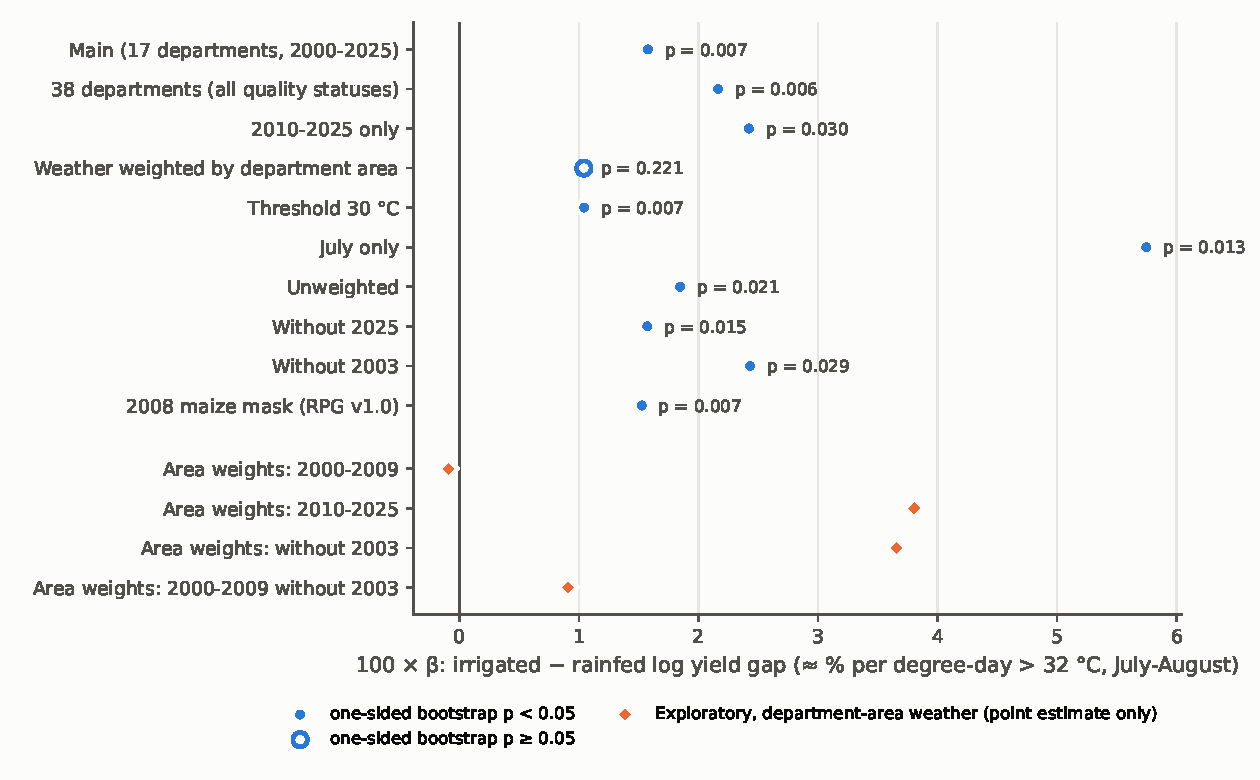
\includegraphics[width=0.95\textwidth]{figures/fig4_mais_robustesse.pdf}
\caption{Coefficient of the main model by specification. Circles: pre-specified and added checks, with the one-sided bootstrap $p$-value; open circle: $p \ge 0.05$. Diamonds: exploratory point estimates with department-area weather, by period, without inference. No intervals are drawn: an interval obtained by inverting the bootstrap was computed for the main specification only (\CiNinetyLow{} to \CiNinetyHigh\,\% at 90\,\%, \cref{subsec:maize-main}), and intervals clustered by year have not had their size checked.}
\label{fig:maize-rob}
\end{figure}

The sign is positive in all \QoneRobN{} specifications and significant in \QoneRobSig. The estimate holds without 2003, the dominant summer; without the provisional year 2025; in the \MaizeDeps{} departments of all quality statuses (\QoneAllDepsPct\,\%); with a 30\,$^{\circ}$C threshold; with July alone; and without weights. With a maize mask drawn from 2008 parcel blocks (grain and silage maize), about eight years older, it is unchanged (\QoneMaskPct\,\%, $p = \QoneMaskP$). One check fails: with weather weighted by the department's surface, the estimate falls to \QoneAreaPct\,\% and is not significant ($p = \QoneAreaP$).

\subsection{Does the result depend on how heat is measured?}
\label{subsec:maize-measure}

Yes, and this is the main limitation of the result. \Cref{tab:maize-measure} shows where the two measures diverge.

\begin{table}[H]
\centering
\small
\caption{Maize: coefficient by heat measure and period (point estimates, exploratory, no inference)}
\label{tab:maize-measure}
% GÉNÉRÉ par scripts/26_tables_memoire.py (phase4bis_q1_exploratoire.csv)
\begin{tabular}{lrr}
\toprule
Period & Maize mask & Department area \\
\midrule
2000--2025 & $+0.0158$ & $+0.0104$ \\
2000--2009 & $+0.0108$ & $-0.0009$ \\
2010--2025 & $+0.0242$ & $+0.0381$ \\
Without 2003 & $+0.0243$ & $+0.0365$ \\
2000--2009 without 2003 & $+0.0380$ & $+0.0091$ \\
\bottomrule
\end{tabular}

\end{table}

The divergence is concentrated in 2000--2009 ($\MaskEarly$ with the maize mask, $\AreaEarly$ with department area) and persists in that decade even without 2003. On 2010--2025, department-wide weather gives a \emph{larger} coefficient (\AreaRecent{} against \MaskRecent).

What we know about the two measures is the following.
\begin{itemize}
  \item \textbf{The age of the mask is not the cause.} A mask drawn from 2008 blocks gives almost the same exposure as the 2015--2017 mask and the same estimate.
  \item \textbf{The department-area measure understates the 2003 heat where maize grows in departments with uplands.} In \ReliefCount{} such departments, maize fields lie \ReliefAltDiffMin{} to \ReliefAltDiffMax{}~m below the department's average altitude, and department-wide weather understates their 2003 heat by up to \ReliefGapMax{} degree-days (\cref{tab:relief}). This is shown for 2003 only, while the divergence persists on 2000--2009 without 2003. An error that scaled heat by the same factor every year would rescale $\beta$, not remove it; removing the association requires errors that reorder departments from one year to the next, which is not shown.
  \item \textbf{Neither measure is checked against where each mode grows.} Both masks assign the same heat to irrigated and rainfed maize. In departments with uplands, irrigated maize may sit lower in the valleys than rainfed maize, so the mask may describe the heat of irrigated fields better than that of rainfed ones.
  \item \textbf{The maize mask was the measure designated in advance} as the main one, before any estimate on 2000--2009 was computed.
  \item \textbf{The choice did not favour the result already known.} When the specification was written, the only known estimate (phase 6, 2010--2025) used department-wide weather and was significant. On those same years the maize mask gives a smaller estimate (\MaskRecent{} against \AreaRecent).
\end{itemize}
These points favour the maize mask. They do not explain the whole divergence, nor why department-wide weather gives a stronger association over 2010--2025, and the altitude pattern was sought after the results were known. Two checks added after the review settle part of this. Dropping one department at a time leaves the estimate between \LooMinPct{} and \LooMaxPct\,\% per degree-day, significant in \LooSig{} cases out of 17. Dropping the six departments with uplands together gives \NoReliefPct\,\% with $p = \NoReliefP$ on the remaining 11: under the rule declared before this check, H1 depends on these departments. Without them the estimate is smaller and less precise; a later check finds no detectable difference between the slopes of the two groups (interaction $+\RelInter$, two-sided $p = \RelInterP$; \cref{subsec:maize-v12}), so the loss of significance is consistent with the remaining 11 departments simply carrying less information. Either way, the significance of the result comes from the very departments where the choice of heat measure matters, which is consistent with the altitude pattern but also means that the measure and the sample cannot be separated. The honest summary is that the result holds when heat is measured where maize is grown, and that it is sensitive to that choice in the earlier decade and rests on the departments with uplands.

\subsection{Is the composition of land moving with heat?}

If hot years changed which land is irrigated, the gap could move for reasons unrelated to irrigation itself. A descriptive check, not pre-specified, is whether the irrigated share of grain maize area moves with heat. With the same fixed effects and controls, one more degree-day above 32\,$^{\circ}$C is associated with a change of $\CompEst$ in the irrigated share ($p = \CompP$, clustered by year, for information only). This check has little power by construction. Areas are largely decided at sowing, before the summer heat, so it cannot detect the more plausible threat: rainfed maize sown for grain but harvested as silage in dry summers, which the yield data do not show; a later descriptive check with the SAA areas of silage maize, available for 2010--2025, finds no detectable increase in the share of rainfed maize harvested as silage in hotter summers (one-sided $p = \SilageP$, mean share \SilageShare\,\%; \cref{subsec:maize-v12}), but this check misses 2003 and silage areas may be recorded before harvest; abandoned fields stay in the statistics with a zero yield. The absence of a detected response is not evidence that composition is stable.

\subsection{What it is worth}

\Cref{tab:valuation} turns the main estimate into quantities for three hot summers. For each department, the extra production associated with irrigation \emph{in a summer hotter than the department's normal} is
\[
\text{irrigated area} \times \text{rainfed yield} \times \big[e^{\hat\beta\,(\ddthirtytwo - \text{department mean})} - 1\big],
\]
valued at the maize price of the year in current euros. Applying the factor to the rainfed yield is the cautious choice; applied to the irrigated yield, the 2003 figure would be about \ValAltPct\,\% higher. The formula extrapolates the linear estimate to 2003, far above the other summers. It also applies to each summer's whole excess heat, national part included, a slope that is identified from differences between departments within a year; in the regression, the national part of each summer is absorbed by the year effects. A simple check suggests it overstates the 2003 figure by about \ValOverPct\,\%: in 2003, the observed gap exceeded each department's average gap by \GapObsTwoThousandThree{} in log terms on average, against \GapPredTwoThousandThree{} predicted by $\hat\beta$.

\begin{table}[H]
\centering
\small
\caption{Production associated with irrigation in hot summers (17 departments, descriptive)}
\label{tab:valuation}
\begin{threeparttable}
{\setlength{\tabcolsep}{4pt}% GÉNÉRÉ par scripts/26_tables_memoire.py (phase4bis_q1_valorisation.csv)
\begin{tabular}{lrrrrrr}
\toprule
Summer & \shortstack{Heat vs.\\normal (DD)} & \shortstack{Irrigated\\area (kha)} & \shortstack{Quintals\\(millions)} & \shortstack{Price\\(EUR/q)} & \shortstack{Value\\(M EUR)} & \shortstack{90\,\% range\\(M EUR)} \\
\midrule
2003 & $+$13.7 & 213 & 2.98 & 16.4 & 49 & 8--98 \\
2019 & $+$2.5 & 195 & 0.43 & 21.3 & 9 & 2--17 \\
2022 & $+$1.9 & 161 & 0.33 & 41.3 & 14 & 3--25 \\
\bottomrule
\end{tabular}
}
\begin{tablenotes}\footnotesize
\item ``Heat vs.\ normal'': area-weighted mean excess of $\mathrm{DD}_{>32}$ over each department's 2000--2025 mean. The range recomputes the value at the bounds of the 90\,\% interval of $\hat\beta$ obtained by inverting the bootstrap by year; it is wide and asymmetric because the bounds enter an exponential. Prices: INSEE index scaled to Eurostat absolute prices over 2012--2016.
\end{tablenotes}
\end{threeparttable}
\end{table}

In the 17 departments, the extra production associated with irrigation in the summer of 2003 is worth about \QoneValTwoThousandThree{} million euros (indicative range \QoneValLow{} to \QoneValHigh). In 2022, fewer quintals are worth more than in 2019 because the price of maize was about twice as high. These figures are gross production values in current euros. They are not the total value of irrigation, which also includes its average advantage; not a value net of the cost of water, energy and labour; not a value per cubic metre or the cost of a water restriction; and not a causal gain. They also leave out the part of the advantage associated with drier soils, since $\beta$ is measured at a given soil wetness.

\subsection{Further checks requested after the audit}
\label{subsec:maize-v12}

A third batch of analyses was declared in the log before being computed, after an internal audit of this text; the log was not committed beforehand, none was pre-specified, and none changes the status of H1. \Cref{tab:maize-v12} summarises them.

\begin{table}[htbp]
\centering
\caption{Maize: further checks (exploratory, declared before computation)}
\label{tab:maize-v12}
\small
\begin{tabular}{p{7.3cm}p{6.2cm}}
\toprule
Check & Result \\
\midrule
\multicolumn{2}{l}{\textit{Inference on H1 ($\hat\beta = \QoneBeta$; bootstrap by year: $p = \QoneP$)}} \\
Cluster jackknife by year (CV3), $t$ with 25 d.f. & one-sided $p = \CvThreeP$ \\
Randomisation inference, 5,000 derangements of years & one-sided $p = \RiP$ \\
Double machine learning (random forests on SWI, P, ETP, growing degree-days; folds by blocks of years) & $\hat\beta = \DmlBeta$, one-sided $p = \DmlP$ \\
\midrule
\multicolumn{2}{l}{\textit{Size of the bootstrap test (300 placebos, nominal 5\,\%)}} \\
H1, heat permuted across departments within each year & \WithinYearSize\,\% \\
H2b (rainfed) and H2c (irrigated), years permuted & \HtwobSize\,\% and \HtwocSize\,\% \\
Placebo Conley matrices corrected by \texttt{fixest} & \ConleyFixedPct\,\% of repetitions \\
\midrule
\multicolumn{2}{l}{\textit{Heterogeneity of the slope}} \\
Heat $\times$ uplands (six departments) & $+\RelInter$, two-sided $p = \RelInterP$ \\
Heat $\times$ irrigated share of grain maize & two-sided $p = \IrrInterP$ \\
Department slopes, empirical Bayes shrinkage & $\tau = \EbTau$, homogeneity $p = \EbQp$; shrunk slopes \EbMin{} to \EbMax \\
Causal forest, calibration test of heterogeneity & $p = \ForestP$ \\
\midrule
\multicolumn{2}{l}{\textit{Other}} \\
Share of rainfed maize harvested as silage, 2010--2025 & no increase with heat, one-sided $p = \SilageP$ \\
Wind capacity and yields \parencite[cf.][]{kaffine2019} & one $p < 0.05$, negative (irrigated yield), not robust to Holm \\
\bottomrule
\end{tabular}
\end{table}

\paragraph{Inference.} The rule of phase 4 bis rests on the bootstrap by year, and it is unchanged. Two other valid procedures do not agree on the strength of the evidence. Randomisation over permuted years gives a smaller $p$-value, but its null leaves the true effect of heat in the error, as the placebo does. The cluster jackknife, which \textcite{mackinnon2023} recommend when clusters are few and unequal in leverage, gives $p = \CvThreeP$: with it, H1 would not be significant at 5\,\%. This is consistent with the concentration of leverage on 2003 (\LevThree\,\% of the weighted residual variation of heat, $N_{\mathrm{eff}} = \NeffLevAll$). The partially linear model of \textcite{chernozhukov2018}, with flexible weather controls, leaves $\hat\beta$ almost unchanged. The new placebo suggested by the review, which keeps each summer's heat in its own year and shuffles it across departments, gives a size of \WithinYearSize\,\%, within the limit of the rule.

\paragraph{Heterogeneity.} None of the three approaches finds a detectable difference in the slope between departments: not by uplands, not by the irrigated share of maize, not by the shrinkage estimator, whose departmental slopes all lie between \EbMin{} and \EbMax{} (they correlate at $\EbCorIrr$ with the irrigated share and $+\EbCorAlt$ with the altitude gap, on 17 points). A causal forest \parencite{athey2019} is uninformative with 435 observations: its calibration test detects no heterogeneity and its average effect is very imprecise. With 17 departments, the data cannot say where the association is stronger.

\paragraph{Variables that were not kept.} The wind capacity installed in each department, built from the national register of electricity installations, is not associated with yields in the way reported for the United States by \textcite{kaffine2019}; the register only lists installations in service in 2026, and departments are too coarse for a local microclimate effect. A satellite measure of surface temperature, which would capture the cooling of irrigated fields \parencite{zhu2022,siebert2017}, was declared but not computed, for lack of access to the NASA service at the time of writing.

\subsection{Summary}

In the main sample, summer heat is associated with a wider yield advantage of irrigated over rainfed maize. The association satisfies the rule fixed before any estimation on 2000--2009, although \ExploSharePct\,\% of its sample comes from the years that suggested it; keeps its sign, with weak evidence, on a decade the exploratory analysis had not used; and survives an older parcel mask and another temperature source. Its magnitude is uncertain and rests largely on 2003; it is not significant without the six departments with uplands (although the slope does not differ detectably between the two groups) or with a cluster jackknife ($p = \CvThreeP$). It depends on measuring heat where maize is grown, a choice made in advance and supported by the geography of the departments concerned, but one that matters. It is an association, not the causal effect of irrigation.

\section{Results: soft wheat, 1959--2025}
\label{sec:wheat}

Wheat was the starting point of the project. Its results are null, but they are instructive: they show what the data can and cannot say, and they motivated the design of the maize analysis. I report them in two steps: the original analysis on 2010--2025, then the extension to 1959--2025.

\begin{figure}[H]
\centering
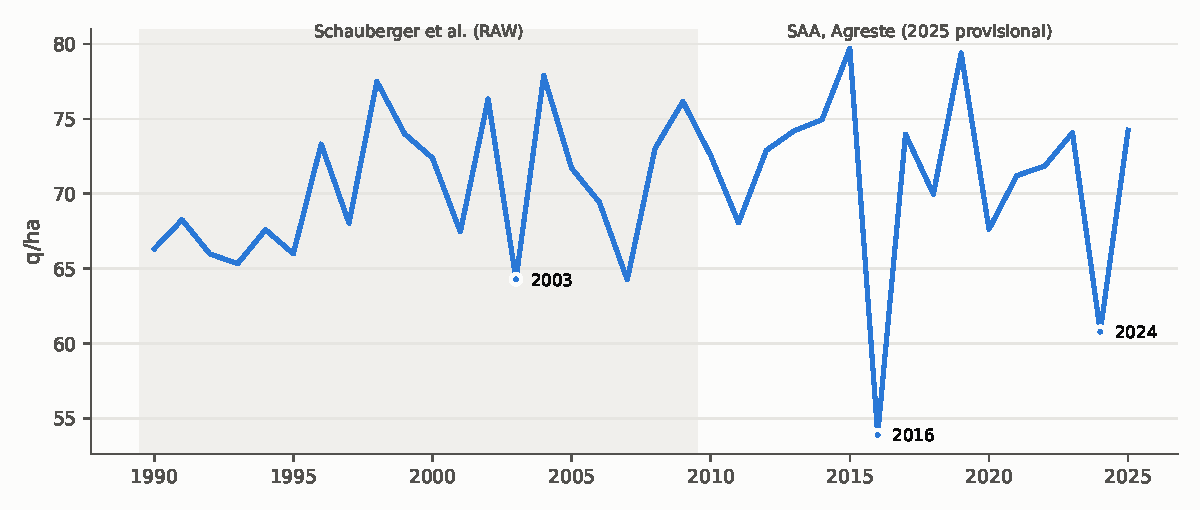
\includegraphics[width=0.95\textwidth]{figures/fig1_rendement_national.pdf}
\caption{Soft winter wheat yield, 1990--2025 (the full series starts in 1959), area-weighted mean of the 85 departments of the population. The shaded period comes from \textcite{schauberger2022}, the rest from the SAA. Yields have plateaued since the mid-1990s, a break also modelled by \textcite{gouache2015}; 2016 and 2024 are the two largest losses since 2010.}
\label{fig:wheat-yield}
\end{figure}

\subsection{2010--2025: a negative association that cannot be established}

\Cref{tab:wheat-short} reports the heat coefficient of the two pre-specified models, with the three inferences planned at the time.

\begin{table}[H]
\centering
\small
\caption{Wheat 2010--2025: heat above 32\,$^{\circ}$C in May--June}
\label{tab:wheat-short}
\begin{threeparttable}
{\setlength{\tabcolsep}{4pt}% GÉNÉRÉ par scripts/26_tables_memoire.py (phase4_principal.csv)
\begin{tabular}{lrrrrrrr}
\toprule
Model & $\hat\beta_2$ & \% per DD & \shortstack{$p$ clust.\\dept.} & \shortstack{$p$\\Conley} & \shortstack{$p$ boot.\\two-sided} & \shortstack{$p$ boot.\\one-sided} & $n$ \\
\midrule
M1 & $-0.0149$ & $-1.48$ & 0.004 & 0.047 & 0.374 & 0.189 & 1328 \\
M2 & $-0.0152$ & $-1.51$ & 0.007 & 0.111 & 0.327 & 0.164 & 1328 \\
\bottomrule
\end{tabular}
}
\begin{tablenotes}\footnotesize
\item M1: equation~\eqref{eq:m1}. M2: M1 plus the May--June soil wetness index and its square. 83 departments, 16 harvests. One-sided: in the direction of the hypothesis $\beta_2 < 0$.
\end{tablenotes}
\end{threeparttable}
\end{table}

Each degree-day above 32\,$^{\circ}$C during grain filling is associated with about \WheatPct\,\% lower yields. The sign is stable:
\begin{itemize}
  \item it is negative in \WheatRobPreNeg{} of the \WheatRobPreTot{} pre-specified robustness checks that change the coefficient (the exception extends the window to July), and in the \WheatRobAddTot{} checks added after the first estimates that estimate the same coefficient (R11--R13; R14 replaces it with temperature bins), defined before being computed;
  \item it is negative in all \LoyoTot{} estimates that leave out one year at a time;
  \item without the provisional year 2025, the association doubles, to about \WheatNoTwentyFivePct\,\% per degree-day.
\end{itemize}

Under the rule fixed in advance, which required all three inferences to agree, the association is not established. The bootstrap by year, the only test whose size was later found to be correct (\cref{sec:inference}), gives $p = \WheatPwcr$. Soil moisture tells the same story: the joint test of the two soil-moisture terms in M2 is highly significant with standard errors clustered by department ($p \WheatHtwoPdep$), and not with the bootstrap by year ($p = \WheatHtwoPwcr$).

This does not show that the effect is absent: the data carry little information on it. With 16 harvests and very hot early summers in only a few of them ($N_{\mathrm{eff}} = \NeffWheat$), a correctly sized test detects a true effect of $-1.5$\,\% only \WheatPowerWCR\,\% of the time (\cref{tab:power}).

\subsection{1959--2025: more years, still not enough}

The natural answer to too few years is more years. Over 1959--2025, the model M3 keeps the variables of M1 and adds department-by-period effects to absorb the breaks between data sources (\cref{sec:strategy}). \Cref{tab:wheat-long} reports the results.

\begin{table}[H]
\centering
\small
\caption{Wheat 1959--2025: heat above 32\,$^{\circ}$C in May--June (83 departments, \QtwoN{} observations)}
\label{tab:wheat-long}
% GÉNÉRÉ par scripts/26_tables_memoire.py (phase4bis_q2_hypotheses.csv, phase4bis_q2_robustesse.csv)
\begin{tabular}{lrrrr}
\toprule
& $\hat\beta_2$ & \% per DD & $p$ boot.\ two-sided & $p$ boot.\ one-sided \\
\midrule
\multicolumn{5}{l}{\emph{Heat slope, M3, and slopes by sub-period}} \\
All years, 1959--2025 (M3) & $-0.0108$ & $-1.08$ & 0.245 & 0.125 \\
Slope 1959--1981 & $-0.0014$ & $-0.14$ & 0.794 & 0.399 \\
Slope 1982--2003 & $-0.0279$ & $-2.75$ & 0.174 & 0.084 \\
Slope 2004--2025 & $-0.0113$ & $-1.13$ & 0.496 & 0.245 \\
\midrule
\multicolumn{5}{l}{\emph{Robustness of the main slope}} \\
Main (M3) & $-0.0108$ & $-1.08$ & --- & 0.125 \\
+ regional linear trends & $-0.0119$ & $-1.18$ & --- & 0.103 \\
Without 2025 (provisional) & $-0.0165$ & $-1.64$ & --- & 0.028 \\
1968--2025 (no missing yields) & $-0.0113$ & $-1.12$ & --- & 0.109 \\
Single department effect & $-0.0113$ & $-1.12$ & --- & 0.112 \\
Threshold 30\,$^{\circ}$C & $-0.0062$ & $-0.62$ & --- & 0.095 \\
\bottomrule
\end{tabular}

\end{table}

\paragraph{The main hypothesis is not established.} The association is \QtwoPct\,\% lower yield per degree-day, close to the estimate on 2010--2025, but a value this negative is not rare when there is no effect: the one-sided $p$-value is \QtwoP. The size of this test on these data is \QtwoSizeWCR\,\%, close to the nominal level in the placebo diagnostic. The sign is negative in all \QtwoRobTot{} robustness checks, and significant in \QtwoRobSig: the one without 2025 (one-sided $p = \QtwoNoTwentyFiveP$, two-sided $\QtwoNoTwentyFivePtwo$). I do not retain it. The rule was fixed in advance, and choosing the variant that ``works'' after seeing the results is exactly what pre-specification is meant to prevent. This sample also contains the 2010--2025 sample, so the similar estimate is not an independent replication.

\paragraph{Why more years did not help much.} Multiplying the number of harvests by four only raised the effective number of informative years from \NeffWheat{} to \NeffWheatLong. Before 2000, only one summer, 1976, brought substantial heat above 32\,$^{\circ}$C in May--June across the sample (\HeatSeventySix{} degree-days on average over the departments, against at most \HeatPreTwoThousandOtherMax{} in any other year before 2000), so most of the added years carry almost no information on it.

\paragraph{Has wheat become more or less sensitive?} The heat slope is $-\SlopeA$\,\% per degree-day over 1959--1981, $-\SlopeB$\,\% over 1982--2003 and $-\SlopeC$\,\% over 2004--2025. The joint bootstrap test that the three slopes are equal gives $p = \QtwoWaldP$; its size was not measured. I find no detectable change, but with so little information this is an absence of evidence, not evidence of stability. Varieties, sowing dates and practices also changed over these decades, so even a detected change would have been descriptive.

\subsection{What the wheat results teach}

Three lessons carried over to the maize analysis. A correct test can be a weak test, and it is better to know it before reading $p$-values. Adding years helps only if the added years contain the shock of interest. And a design that compares two outcomes exposed to the same summer, such as irrigated and rainfed maize in the same department, removes much of the common variation that makes the wheat estimates so imprecise.

\section{Forecasting wheat yields}
\label{sec:forecasting}

The econometric question asks whether heat is associated with yields. A separate, practical question is whether the weather known before harvest helps to predict them. This section answers it with a strictly chronological protocol. The answer is no, at least not better than the simplest benchmark.

\subsection{Protocol}

The protocol was fixed in a specification written before any forecast was computed (\cref{tab:specs}).
\begin{itemize}
  \item \textbf{Target and sample.} The log yield of soft wheat in the 83 departments of the main sample.
  \item \textbf{Forecast dates.} 1 June and 1 July of the harvest year. Only weather up to the day before is used: autumn, winter, spring, and May (on 1 June) or May--June (on 1 July). Nine variables per window give 36 variables, fixed in advance.
  \item \textbf{Validation.} Rolling origin: for each test year $t$ from 2016 to 2025, models are trained on 2010 to $t-1$, between 6 and 15 years. Department means, trends, standardisation and hyperparameters are all estimated within the training years. A variant trains from 1990 with the long wheat series.
  \item \textbf{Benchmarks.} B0 is the mean log yield of the department over the training years. B1 adds a common linear trend.
  \item \textbf{Models.} Each model predicts the residual of B1 from the weather variables: ordinary least squares on the variables of model M1, ridge regression, a random forest and gradient boosting. Their settings were fixed in advance; only the ridge penalty is tuned, by an inner leave-one-year-out loop on the training years.
  \item \textbf{Uncertainty.} The difference in mean squared error between a model and a benchmark is given with a 95\,\% interval from a block bootstrap over the 10 test years.
\end{itemize}
Tests check automatically that no variable uses information from after the forecast date. Some leakage cannot be removed: the SAA series were revised after the 2020 census, SIM is a reanalysis, the wheat mask comes from 2015--2017, and the 2025 yields are provisional. The sample itself is chosen with information later than some test years (the quality status published in 2025), so the exercise is a pseudo-real-time test, not a real-time one. Two smaller points: the degree-days of the last day before the forecast date use the next day's minimum temperature, which SIM measures until 18:00 UTC on the forecast day itself; and the inner loop that tunes the ridge penalty leaves out one training year at a time, so it uses training years later than the one left out. The first adds a few hours of weather after the forecast date; neither uses the yields of the test year.

\subsection{The benchmark that matters}

The specification compared models with B1. Under that pre-specified criterion, the random forest on 1 July formally qualifies as a gain: a skill of \RfVsBoneSkill\,\% with an interval excluding zero. But B1 turned out to be a weak benchmark: B0, the plain department mean, beats B1 in all \BzeroBeatsBone{} test years, because French wheat yields have plateaued (\cref{fig:wheat-yield}), so extending a trend hurts. I decided, after seeing these results, to add the comparison with B0, a benchmark already defined in the specification, and logged this change (\cref{app:deviations}). The results against B1 remain in the project tables.

There is a second consequence. The weather models were built, as specified, as corrections to B1, so they inherit its handicap: B1 itself is far worse than B0 (\cref{tab:forecast}). The comparison below therefore tests the models as pre-specified, not the value of weather as such. A model that corrects B0 instead of B1 was evaluated afterwards, on the same test years (\cref{subsec:forecast-v12}); it can only suggest what to test on new years.

\subsection{Results}

\begin{table}[H]
\centering
\small
\caption{Forecast skill relative to the department mean (B0), test years 2016--2025}
\label{tab:forecast}
\begin{threeparttable}
% GÉNÉRÉ par scripts/26_tables_memoire.py (phase5_synthese_vs_B0.csv)
\begin{tabular}{llrrr}
\toprule
Date & Model & \shortstack{Skill vs.\\B0 (\%)} & \shortstack{95\,\% interval of MSE\\difference ($\times 10^3$)} & \shortstack{Years better\\than B0} \\
\midrule
\multicolumn{5}{l}{\emph{Train from 2010}} \\
1 June & B1 (trend) & $-36$ & [$+1.2$, $+19.6$]$^*$ & 0/10 \\
1 June & OLS (M1 variables) & $-53$ & [$+3.4$, $+22.9$]$^*$ & 2/10 \\
1 June & Ridge & $-27$ & [$-1.4$, $+16.8$] & 5/10 \\
1 June & Random forest & $-15$ & [$-5.8$, $+15.2$] & 5/10 \\
1 June & Gradient boosting & $-24$ & [$-4.2$, $+18.0$] & 5/10 \\
1 July & B1 (trend) & $-36$ & [$+1.3$, $+19.7$]$^*$ & 0/10 \\
1 July & OLS (M1 variables) & $-72$ & [$+4.9$, $+31.9$]$^*$ & 1/10 \\
1 July & Ridge & $-59$ & [$-3.6$, $+36.0$] & 4/10 \\
1 July & Random forest & $-14$ & [$-5.7$, $+14.9$] & 5/10 \\
1 July & Gradient boosting & $-22$ & [$-3.7$, $+15.3$] & 4/10 \\
\multicolumn{5}{l}{\emph{Train from 1990}} \\
1 June & B1 (trend) & $-18$ & [$-1.1$, $+11.6$] & 4/10 \\
1 June & OLS (M1 variables) & $-17$ & [$-2.8$, $+14.0$] & 6/10 \\
1 June & Ridge & $+9$ & [$-4.3$, $+0.3$] & 7/10 \\
1 June & Random forest & $+9$ & [$-8.1$, $+3.5$] & 5/10 \\
1 June & Gradient boosting & $+7$ & [$-7.0$, $+3.6$] & 5/10 \\
1 July & B1 (trend) & $-18$ & [$-1.2$, $+11.4$] & 4/10 \\
1 July & OLS (M1 variables) & $-21$ & [$-0.8$, $+13.9$] & 3/10 \\
1 July & Ridge & $+20$ & [$-16.0$, $+2.4$] & 3/10 \\
1 July & Random forest & $+11$ & [$-7.8$, $+2.2$] & 5/10 \\
1 July & Gradient boosting & $+13$ & [$-6.5$, $+0.6$] & 7/10 \\
\bottomrule
\end{tabular}

\begin{tablenotes}\footnotesize
\item Skill $= 1 - \mathrm{MSE}/\mathrm{MSE}(\mathrm{B0})$, on log yield, weighted by area. Interval: 95\,\% block bootstrap over test years; $^*$: excludes zero. Positive values in the interval mean worse than B0.
\end{tablenotes}
\end{threeparttable}
\end{table}

\Cref{tab:forecast} gives the answer.
\begin{itemize}
  \item \textbf{Training from 2010:} every model does worse than B0 on average, by \ForecastBestPct\,\% to \ForecastWorstPct\,\%, and the OLS model is significantly worse.
  \item \textbf{Training from 1990:} ridge, random forest and gradient boosting do better than B0 on average, but their intervals include zero over 10 test years.
\end{itemize}
No model, as pre-specified, is significantly better than the department mean.

\begin{figure}[H]
\centering
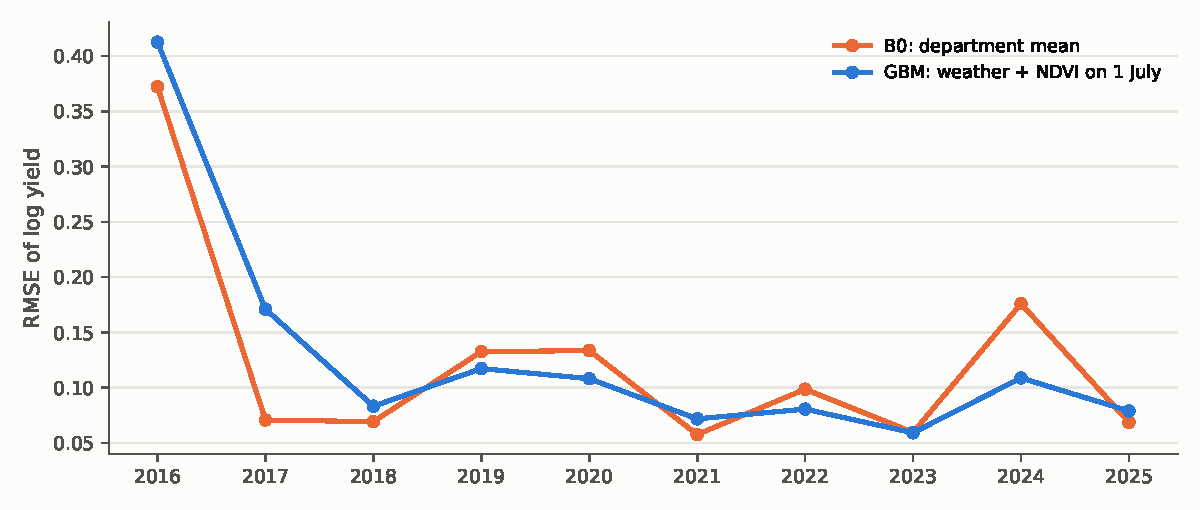
\includegraphics[width=0.95\textwidth]{figures/fig3_prevision_par_annee.pdf}
\caption{Forecast error by test year on 1 July: department mean (B0) and gradient boosting with weather and NDVI. Each model is trained only on the years before the test year.}
\label{fig:forecast-year}
\end{figure}

\subsection{Adding satellite data}

A natural objection is that weather describes the conditions, not the crop. The NDVI, a satellite index of green vegetation, describes the crop itself. I added MODIS NDVI at 250~m (16-day composites from April to June), aggregated to SIM cells and then to departments with the wheat mask. A composite is used only if it ends before the forecast date, a rule checked by an automated test.

\begin{table}[H]
\centering
\small
\caption{What NDVI adds to each model, training from 2010}
\label{tab:ndvi}
\begin{threeparttable}
% GÉNÉRÉ par scripts/26_tables_memoire.py (phase6_ndvi_synthese.csv)
\begin{tabular}{llrrr}
\toprule
Date & Model & \shortstack{Gain from NDVI vs.\\same model (\%)} & \shortstack{95\,\% interval of MSE\\difference ($\times 10^3$)} & \shortstack{Skill vs.\\B0 (\%)} \\
\midrule
1 June & Ridge & $+1.6$ & [$-1.55$, $+0.64$] & $-25$ \\
1 June & Random forest & $+1.6$ & [$-0.85$, $-0.11$]$^*$ & $-13$ \\
1 June & Gradient boosting & $+3.5$ & [$-2.26$, $-0.02$]$^*$ & $-20$ \\
1 July & Ridge & $+27.7$ & [$-22.44$, $-1.08$]$^*$ & $-15$ \\
1 July & Random forest & $+1.6$ & [$-0.95$, $+0.01$] & $-13$ \\
1 July & Gradient boosting & $+7.6$ & [$-4.55$, $-0.26$]$^*$ & $-12$ \\
\bottomrule
\end{tabular}

\begin{tablenotes}\footnotesize
\item Gain: $1 - \mathrm{MSE}(\text{with NDVI})/\mathrm{MSE}(\text{without})$. Interval of the MSE difference with minus without; $^*$: excludes zero (here, always better with NDVI).
\end{tablenotes}
\end{threeparttable}
\end{table}

NDVI helps each model a little: the gain over the same model without NDVI is positive in all \NdviTot{} cases, from \NdviGainMin{} to \NdviGainMax\,\%, and significant in \NdviSig. The largest gain, for ridge on 1 July, mostly reflects the stabilisation of a model that was unstable without NDVI. But no model with NDVI does better than the department mean, even on average (\cref{tab:ndvi}, last column). The NDVI is measured on 8~km cells weighted by wheat, not on wheat parcels alone, so it mixes crops; a parcel-level index might do better.

\subsection{What the forecasting results mean}

With 6 to 15 training years, the models as pre-specified are not significantly better than a well-chosen naive benchmark, and NDVI adds a small measurable improvement to each of them without changing that conclusion. This is consistent with earlier warnings that validation on future years is much harder than cross-validation \parencite{gouache2015,morales2023}. The main methodological point is the benchmark: had I kept the pre-specified comparison with B1 alone, I would have reported a forecasting gain over B1 that is not a gain over the simplest forecast. Whether weather can improve on B0 itself remains open.

\subsection{Correcting the department mean, and prediction intervals}
\label{subsec:forecast-v12}

The previous section left open whether weather can improve on B0. Two analyses added later, each declared in the log before it was computed, address it; both use test years that had already been seen, so they are exploratory. First, tree models built as corrections to B0 instead of B1, with the same 36 variables and the same settings, do better than B0 by \BzeroTreeMin{} to \BzeroTreeMax\,\% in mean squared error, with a 95\,\% interval that excludes zero in \BzeroTreeSig{} of the 4 cases (random forest on both dates, gradient boosting on 1 July); ridge regression does worse. This is the most promising forecasting result of the project, but it was found after B1 had been seen to fail on the same years, and it needs confirmation on the harvests from 2026, with this protocol frozen. Second, split conformal intervals \parencite{lei2018}, recalibrated each year on the residuals of earlier test years, cover \ConfCovMin{} to \ConfCovMax\,\% of departments for a nominal 90\,\%, so they are too wide: the quantile is dominated by the 2016 loss, and with so few years the intervals are not calibrated.

\section{Discussion}
\label{sec:discussion}

This section asks three questions. What does the maize result mean, and what could make it wrong? How far does it travel beyond the 17 departments studied? And what did the way the project was run teach, independently of its results?

\subsection{What the maize result means}

In the main sample, irrigated maize keeps about \IrrShareOfRainfedSens\,\% of the heat sensitivity of rainfed maize: about $-$\QoneIrrigatedPct\,\% per degree-day above 32\,$^{\circ}$C against $-$\QoneRainfedPct\,\%. The direction matches studies abroad, which find a much smaller heat sensitivity for irrigated than for rainfed maize in the United States \parencite{schauberger2017} and, for wheat in India, about a quarter of the rainfed sensitivity \parencite{zaveri2019}. The data, crops and designs differ too much for a closer comparison of magnitudes.

Two features of the result deserve emphasis. Irrigation is associated with a smaller sensitivity to heat, not with its disappearance: irrigated maize still loses yield in hot summers. And the association rests largely on a few summers, above all 2003, which carries between a quarter and two fifths of the useful variation in heat, depending on whether weights and soil moisture are taken into account (\cref{sec:exposure,subsec:maize-inference}). This is why the strength of the evidence depends on the inference: the bootstrap by year rejects, the more conservative cluster jackknife does not. A linear effect per degree-day is a convenient summary, not a law: in 2003 the observed widening of the gap was smaller than the linear estimate predicts (\cref{sec:maize}).

\paragraph{Heat, or hot and dry summers.} In France the summers with many degree-days above 32\,$^{\circ}$C (2003, 2019, 2022) were also dry. The soil wetness index absorbs part of this, but it comes from a land-surface model whose documentation does not mention irrigation, and the result holds when it is dropped or replaced by a climatic water balance (\cref{sec:maize}), but heat and the water balance remain correlated. ``Heat'' in this monograph therefore means hot, and mostly dry, summers. The vapour pressure deficit makes this precise: in a model with both, the association moves from degree-days above 32\,$^{\circ}$C to the drying power of the air (\cref{subsec:maize-vpd}), as \textcite{lobell2013} found for American maize. The two are too correlated to be separated here, but the safest reading of the main result is that irrigated maize resists hot, dry summers better, more than that it resists heat as such. Whether irrigation helps by supplying water or also by cooling the canopy cannot be told apart with these data. Satellite studies elsewhere attribute about a third of the benefit of irrigation to cooling \parencite{zhu2022}, and heat stress computed from air temperature overstates the stress of irrigated crops \parencite{siebert2017}; with air temperature common to both modes, as here, part of what is called heat may be the absence of this cooling on rainfed fields. A check with MODIS surface temperature is consistent with this reading without settling it: across the 38 departments, surface temperature rises by about \LstSlope{}\,$^{\circ}$C per degree-day above 32\,$^{\circ}$C, a little less where more maize is irrigated (\LstSlopeQone{} at the first quartile of the irrigated share, \LstSlopeQthree{} at the third; two-sided $p = \LstInterP$), but the irrigated share also differs across departments in other ways.

\paragraph{Water restrictions.} The pre-specified interaction with crisis-level restrictions has the opposite sign to the hypothesis (\cref{sec:maize}). It is read descriptively, as planned, and it gives no support to the idea that restrictions reduced the advantage of irrigated maize in these departments.

\subsection{What could make it wrong}

The estimate is an association within departments and years. For it to measure how irrigation changes the response to heat, irrigated and rainfed land would have to differ only in ways that do not themselves vary with the heat of the summer. Several mechanisms could break this.

\paragraph{Silage.} In a hot, dry summer, some rainfed maize sown for grain may be harvested as silage instead. Abandonment is less of a concern: the SAA counts unharvested area with a zero yield, so abandoned fields stay in the grain statistics. Silage is different. If the worst rainfed fields move from grain to silage, the observed rainfed grain yield is the yield of the remaining fields and overstates what rainfed maize produced. Under that assumption, this would bias the gap downwards in hot years, against the result; if the fields moved to silage are not the worst ones, the direction of the bias is not known. The SAA areas of silage maize, available for 2010--2025, show no detectable increase in the share of rainfed maize harvested as silage in hotter summers (\cref{subsec:maize-composition}), but 2003 is outside that period and the areas may be recorded before harvest. The irrigated share of grain maize area does not move detectably with heat (\cref{sec:maize}), but areas are largely decided at sowing, so this check cannot see the mechanism.

\paragraph{Irrigation itself responds to heat.} Farmers irrigate more in hot summers, unless restrictions stop them. The estimate therefore mixes the agronomic effect of water with the behavioural response of irrigators. This is part of what ``irrigated maize'' means in practice, and it is why the result describes the observed advantage of irrigated maize, not the effect of a fixed amount of water.

\paragraph{Other changes in the departments.} The year effects absorb national trends, not changes specific to a department that would move with its summers. One such change was examined: wind farms, which an American study associates with higher nearby yields through their effect on local climate \parencite{kaffine2019}. Onshore wind capacity per hectare of farmland, built from the national register of electricity installations, shows no positive association with irrigated, rainfed or wheat yields and does not move the gap. Its one coefficient with $p < 0.05$, for irrigated maize, is negative and does not survive a correction for the four tests. The test is weak in any case: the register lists only installations in service in 2026, and departments are too coarse for a local effect.

\paragraph{Different land, different farms.} Irrigated fields tend to be on soils and farms suited to intensive maize. Department fixed effects absorb the stable part of these differences. They would not absorb, for example, a tendency of better farms to protect their irrigated maize more in hot years.

\paragraph{Measurement.} Four sources of error are documented in the monograph:
\begin{itemize}
  \item the result depends on measuring heat where maize grows (\cref{sec:maize});
  \item SIM2 is an 8~km reanalysis; E-OBS, interpolated from stations, counts more degree-days above 32\,$^{\circ}$C, and the result holds with both;
  \item the masks do not distinguish irrigated from rainfed parcels, so both modes are assigned the same heat;
  \item fixed calendar windows ignore year-to-year shifts in crop development \parencite{leroux2024}.
\end{itemize}
Errors in heat that are unrelated to the gap would bias $\beta$ towards zero, and instrumenting the SAFRAN measure by E-OBS raises the estimate by about a third (\cref{subsec:maize-measure}); errors that differ systematically between irrigated and rainfed land have no known direction.

\paragraph{The data on yields.} The quality status of 2025 is applied to 2000--2009, two releases of the statistics are spliced in 2010, many yields are rounded, and the 2025 values are provisional. The splice was checked on the overlap and the results do not depend on 2025, but the older decade rests on a release that was never revised.

\paragraph{How the split between irrigated and rainfed maize is produced.} The SAA is a synthesis of several sources, compiled by regional statistical services. This monograph does not document how they set the irrigated and rainfed yields separately, nor whether ``irrigated'' means land actually irrigated that year or land equipped for irrigation. If part of the split were estimated from expert judgement about dry summers, the gap could reflect the estimation method as much as the harvest. This was flagged when the project was scoped and remains the main untested limitation of the outcome variable.

\subsection{How far the result travels}

The main sample covers \MainShareArea\,\% of the maize area of the population, and within it the significance of the association rests on the six departments with uplands: without them it is not significant, although their slope does not differ detectably from that of the others (\cref{subsec:maize-measure}). It is concentrated in Alsace, the Rhône--Alpes and Auvergne area, the Centre and Burgundy--Franche-Comté. It excludes the South-West (Landes, Pyrénées-Atlantiques, Gers, Lot-et-Garonne, among others), France's main maize basin, and the Centre-West (Charente, Charente-Maritime, Deux-Sèvres, Vendée, Vienne), whose irrigated series have a lower quality status. With all 38 departments, the estimate is larger (\QoneAllDepsPct\,\% per degree-day) and significant, which is reassuring but rests on data the statistics office itself rates lower. Beyond grain maize, the same association appears for silage maize in \FodderDeps{} departments over 2010--2025 (\FodderPct\,\% per degree-day), so it is not specific to one crop's statistics.

The estimand also limits extrapolation in time. It describes the response to a hot summer given current varieties, practices and water rules. A lasting rise in temperature would bring adaptation, in sowing dates, varieties and the extent of irrigation, and possibly tighter water restrictions. Whether panel estimates of this kind approximate such long-run responses depends on conditions studied by \textcite{merel2021}; I do not claim that they hold here.

\subsection{What would settle the open questions}

\begin{itemize}
  \item \textbf{A map of irrigated parcels.} Assigning heat separately to irrigated and rainfed fields would remove the main measurement limitation. The parcel register used here does not record irrigation; maps derived from Sentinel-1 and Sentinel-2 exist for some basins, not for the whole country.
  \item \textbf{Surface temperature on irrigated and rainfed fields separately.} The MODIS check above averages both modes within each pixel; combined with a map of irrigated parcels, surface temperature would show directly whether irrigated fields stay cooler in hot summers \parencite{zhu2022}.
  \item \textbf{How the SAA splits irrigated and rainfed maize.} The public descriptions of the SAA do not say whether ``irrigated'' means irrigated that year or equipped for irrigation. The statistical service could answer it, and its farm-practice surveys, which record irrigation and yield field by field, could validate the split at the regional level.
  \item \textbf{Data on maize moved from grain to silage in dry years.} The SAA areas of silage maize show no shift over 2010--2025; field-level data on the harvest decision, and data covering 2003, would test the main selection threat directly.
  \item \textbf{Water volumes.} The national register of water withdrawals offers annual irrigation volumes for 2012--2023 for all water agencies, but for all crops together and with breaks in reporting; I audited this source for the project but did not use it. It could support a descriptive value per cubic metre in departments where maize dominates irrigation, not an estimate of the productivity of water.
  \item \textbf{More hot summers.} The information on heat grows only when hot summers occur. Re-estimating the model as new harvests are published, with the specification unchanged, is the cleanest test of the result.
\end{itemize}

\subsection{What the way of working taught}

Three lessons are independent of the results.

\paragraph{Check the size of your tests on your data.} The usual standard errors would have made the wheat result look solid ($p = \WheatPdep$ instead of $\WheatPwcr$). A placebo with permuted years costs a few minutes and changed the conclusions of this project. It does not detect every problem (serial correlation is one it cannot see), but it is a check that panels with common shocks should not skip. Nor should a single valid test be the end of it: when one year dominates, as 2003 does, other valid inferences can disagree, and reporting them is part of the result.

\paragraph{Choose the benchmark before the model.} In forecasting, the pre-specified trend benchmark was weaker than the plain department mean. Judged against it, a model looked useful when it was not. The comparison that matters is with the simplest forecast a user would otherwise make.

\paragraph{Pre-specification helps, within limits.} Writing the specification first, with its hash in a log, made it visible, and costly, to choose the variant that worked: the wheat result without 2025 was significant in the one-sided test and was not retained. It did not make the work blind, and it was not timestamped by anyone but the author: the specifications entered the public repository together with the first results. The maize question was chosen after an exploratory analysis, some checks were added after results were known, and one departure went unnoticed until a review. Saying so, and listing every departure (\cref{app:deviations}), is part of what makes the remaining claims credible.

\section{Conclusion}
\label{sec:conclusion}

In 17 French departments over 26 summers, extreme heat in July and August is associated with a wider yield advantage of irrigated over rainfed grain maize: \QonePct\,\% per degree-day above 32\,$^{\circ}$C, with a test whose size was checked on the same data. Rainfed yields are about \QoneRatio{} times more sensitive to heat than irrigated yields, which are themselves not immune. The association met a decision rule fixed before the replication years were seen, kept its sign on a decade the exploratory analysis had not used, with an estimate about half the 2010--2025 one, and did not change with an older map of maize. It depends on measuring heat where maize is grown, and in the earlier decade it does not hold with department-wide weather. It is an association, not the causal effect of irrigation, and it says nothing direct about a warmer climate.

The other questions gave null results. For wheat over 1959--2025, heat at the end of the cycle is associated with lower yields, but this cannot be distinguished from zero, and no change in sensitivity over time is detectable. Forecasts of wheat yields from weather and satellite data, as pre-specified, are not significantly better than the historical mean of each department.

The most general finding is methodological. In panels where a weather shock hits many units in the same year, standard errors clustered by unit or with a spatial cut-off can reject a true null in a large share of cases: \UsualSizeMin\,\% to \UsualSizeMax\,\% here. A placebo that keeps the real geography of the shock and permutes years reveals the problem in minutes. The code for this check is released with the monograph, so that it can be run on other data before their conclusions are drawn.


\clearpage
\printbibliography[heading=bibintoc]

\clearpage
\appendix
\section{Reproduction}
\label[appendix]{app:reproduction}

Everything in this monograph can be rebuilt from public sources with the project's code. The code is available at \url{https://github.com/maxime2476/Atlas} and archived on Zenodo (\href{https://doi.org/10.5281/zenodo.23305095}{doi:10.5281/zenodo.23305095}). This appendix says how, and what is needed.

\paragraph{Environments.} Python~3.12 is managed with \texttt{uv}. Its lock file fixes every package, resolved with no release later than \VerUvDate{} (for instance pandas~\VerPandas, scikit-learn~\VerSklearn, DuckDB~\VerDuckdb, GeoPandas~\VerGeopandas). R~\VerR{} is managed with \texttt{renv}, from a dated snapshot of the Posit package repository (\VerRepoDate), with \texttt{fixest}~\VerFixest. The two languages exchange data through Parquet files with documented schemas.

\paragraph{Raw data.} About \RawSizeGb~GB of raw files, never modified, of which \DriasSizeGb~GB of climate projections (NDVI, E-OBS and DRIAS included). A manifest lists \ManifestFiles{} files with their URL, access date and SHA-256 hash; an automated test checks every hash. The raw data are not redistributed with the code; the download script rebuilds them.

\paragraph{Pipeline.} The repository's \texttt{data/README.md} gives the commands in order:
\begin{enumerate}
  \item downloads and checks;
  \item weather, crop masks, exposure windows and panels;
  \item econometrics in R;
  \item forecasting and NDVI;
  \item the pre-specified analyses of phase 4 bis;
  \item the checks added later, including soils, irrigation volumes and climate projections;
  \item figures, then the tables and figures of this monograph.
\end{enumerate}
The longest steps are the NDVI processing (orders depend on the NASA queue, then about 15 minutes of aggregation and 30 minutes of forecasting) and the daily weather (about 20 minutes). Two sources require a free personal account: the NDVI (NASA Earthdata) and the climate projections (DRIAS and DRIAS-Eau, one account for both). DRIAS has no download interface: orders are placed through its web form, by a script that fills it in as a user would, and are delivered later as archives. Its terms forbid sharing the account, so a reproduction needs its own; the projections are therefore the one step that cannot be rebuilt without registration. All other sources are open without registration.

\paragraph{A clean rebuild.} Before the checks added later, the whole chain was run again on a fresh copy of the repository, from the raw files and without downloading anything. It gave the same intermediate data, the same result tables byte for byte (except the forecast tables, which differ by at most $5\times 10^{-15}$, floating-point rounding) and the same numbers as the text at that point. The analyses added afterwards (all those marked as added later in \cref{sec:maize,sec:forecasting}, and the projections of \cref{sec:discussion}) were run in the working repository, not on a fresh copy.

\paragraph{The numbers in this text.} Every estimate, $p$-value, test size and table in this monograph is generated: a script reads the result tables of the project and writes them as \LaTeX{} macros and tables. A few numbers are written in the text by hand: counts that define the design (17 and 83 departments, the numbers of years and clusters, the 300 placebo repetitions) and a few historical figures from the decision log, which are cited as such. The script also checks that the specifications still match their recorded hashes and that the valuation of 2003 is reproduced exactly; it stops otherwise.

\paragraph{Tests.} The test suite has \TestCount{} tests: \TestIntegrity{} integrity checks of the raw files, one per file, and \TestLogic{} tests of logic and data. Together they check schemas, keys, the cardinality of joins, value ranges, the degree-day formula, the absence of forecasting leakage, the agreement of the maize mask with official statistics, and the integrity of the raw files. Tests that need data are skipped when the data are absent. The R code has no unit tests; it is validated by comparisons with \texttt{fixest} and by the size simulations of \cref{sec:inference}.

\paragraph{Randomness.} All random draws use fixed seeds, recorded in the code. One departure from the seed written in the phase 4 bis specification is listed in \cref{app:deviations}.

\section{Variable dictionary}
\label[appendix]{app:variables}

\begin{table}[H]
\centering
\footnotesize
\caption{Main variables}
\label{tab:variables}
\begin{tabular}{>{\raggedright}p{3.2cm}>{\raggedright}p{6.9cm}>{\raggedright}p{1.6cm}>{\raggedright\arraybackslash}p{2.1cm}}
\toprule
Variable & Definition & Unit & Source \\
\midrule
Yield $Y$ & Production over area (unharvested area counted with a zero yield), by department, crop and, for maize, irrigation mode & q/ha (1~q = 100~kg) & SAA; \textcite{schauberger2022} \\
Gap & $\ln Y^{I} - \ln Y^{R}$, same department and year & log points & SAA \\
$\mathrm{DD}_{>32}$ & Degree-days above 32\,$^{\circ}$C by double sine, summed over the window, crop-weighted mean of cells & $^{\circ}$C$\cdot$day & SIM2, RPG \\
GDD & Degree-days between 0 and 32\,$^{\circ}$C ($\mathrm{DD}_0 - \mathrm{DD}_{32}$) & $^{\circ}$C$\cdot$day & SIM2, RPG \\
SWI & Soil wetness index, mean over the window (about 0 at wilting point, 1 at field capacity) & none & SIM2 \\
$P$ & Precipitation (rain and snow), summed over the window & mm & SIM2 \\
Crisis days & Days of July--August with at least one zone of the department at crisis level & days & VigiEau \\
Weights & Mean area 2010--2012 (wheat; or irrigated plus rainfed grain maize) & ha & SAA \\
Windows (wheat) & Autumn: Sep--Nov of $t-1$; winter: Dec--Feb; spring: Mar--Apr; grain filling: May--Jun & --- & --- \\
Window (maize) & July--August & --- & --- \\
NDVI & Mean and maximum of 16-day composites, April--June, only if ended before the forecast date & none & MODIS \\
\bottomrule
\end{tabular}
\end{table}

\section{Deviations from the pre-specified plans}
\label[appendix]{app:deviations}

The project's decision log records every change to the plans, with its date and reason. This appendix lists them by phase. ``Declared before'' means the change was written in the log before the corresponding estimate was computed. The work ran in four stages: first the pre-specified analyses of each phase; then, once the whole text existed, a later stage of checks requested in a simulated review of it; then a stage after an internal audit; and, last, two checks requested by four simulated reviews of the finished text. The checks of the three later stages are marked as added later in the text.

{\footnotesize
\renewcommand{\arraystretch}{0.97}
\begin{longtable}{>{\raggedright}p{1.3cm}>{\raggedright}p{7.3cm}>{\raggedright\arraybackslash}p{4.6cm}}
\caption{Deviations and additions, by phase (from the project's decision log)}
\label{tab:deviations} \\
\toprule
Phase & Change & Timing and effect \\
\midrule
\endfirsthead
\toprule
Phase & Change & Timing and effect \\
\midrule
\endhead
Long series & \textcite{schauberger2022}: RAW version used instead of FILTERED, although the compatibility criterion had been written for FILTERED; the filter mostly masks years of real losses, so using it would select on the outcome & Logged before any estimate of a weather effect; affects the long wheat panels \\
4 (wheat) & Joint test of the soil-moisture terms under the bootstrap by year; one-sided bootstrap $p$-value for H1 & Planned tests initially omitted, added before interpretation \\
4 & Two-sided 95\,\% interval for H1, planned in the specification & Omission found by an internal review; computed in a later stage: $\WheatCiLow$ to $+\WheatCiHigh$\,\% per DD \\
4 & Individual bootstrap test on the first soil-moisture term declared not interpretable (slope outside the observed support); test on the second term added & Not pre-specified \\
4 & Leave-one-year-out estimates; size and power simulation with a placebo (years permuted) & Not pre-specified; added after the first estimates; reported as diagnostics \\
4 & Four robustness checks R11--R14 (shifted windows, mountain departments, temperature bins) & Added after the first estimates; defined in the log before being computed \\
4 & Two bugs: bootstrap outcome not re-projected (size 8.7\,\% $\to$ 6.6\,\%); operator precedence in the simulation script & Corrected before any interpretation \\
4 & Conley matrices that \texttt{fixest} had to correct (not positive definite) & $p$-values set to missing, not reported \\
5 (forecast) & Comparison with B0 added and put first, because B1 turned out to be weaker than B0 & Decided after seeing results; B1 results still reported \\
6 (explor\-atory) & Two maize observations with zero irrigated area dropped; size check on maize & Not foreseen in the specification; reported as such \\
6 & NDVI protocol (product, quality filter, aggregation, availability rule) & Fixed before the data were received \\
6 & Missing NDVI values ($\leq 1.1\,\%$ per variable) imputed within each fold by the department's training mean & Not foreseen in the protocol; logged before results \\
4 bis (maize) & Population: 2025 quality status applied to 2000--2009 & Declared before estimation (no earlier status exists) \\
4 bis & Factual correction: 18 missing wheat yields in the main sample, not 27 (27 is the count for the population) & Logged before estimation; model unchanged \\
4 bis & Execution fixes: outcome variable of the maize size simulation, columns of a wheat table; Conley $p$-values set to missing for several maize terms & No effect on the models \\
4 bis & Seed of the bootstrap 20261010 instead of 20261011 & Not declared; found by the internal review; Monte Carlo error $\approx 0.002$ on $p$ near 0.05 \\
4 bis & Robustness check with a 2008 mask of maize parcel blocks (Q1-R9) & Declared before estimation, after the internal review of phase 0 ter; reading rule fixed in advance \\
4 bis & Power; replication size; E-OBS heat; after a simulated review: interval of $\beta$, departments, moisture, decades & Later stage, after a simulated review; each logged before computation \\
4 bis & After the audit: inference variants (CV3, randomisation, DML), within-year placebo, sizes of H2b--H2c, leverage, slope heterogeneity (interactions, shrinkage, causal forest), silage, wind; MODIS surface temperature (protocol fixed before the data were received); silage-maize replication, timing placebos, instrumental variables, non-linearity, heat $\times$ soil moisture, vapour pressure deficit; frozen specification for future harvests; vapour pressure deficit on silage maize, years dropped one at a time, serial-correlation simulation, specification curve; soil water capacity, irrigation volumes, value per cubic metre (with a dose plausibility rule); projections of heat under the French warming levels (DRIAS) & Last stage, after an internal audit; each logged before computation; exploratory \\
4 bis & After four simulated reviews of the text: size and power of the cluster jackknife (V1); signatures of imputation in the irrigated--rainfed split, with a conditional re-estimation (V2) & Declared before computation, with reading rules; descriptive \\
4 bis & Also suggested by the reviews: heat averaged over SIM2 and E-OBS (P1), slopes by quality status (P2), soil wetness in the projections (P3), a first look at the 2026 harvest from early estimates and registration of the frozen wheat forecast for 2026 (P4) & Declared before computation, with reading rules; exploratory \\
4 bis & Improvement checks: leverage of each year and wild bootstrap of the cluster-jackknife statistic (L1), estimate without the repeated irrigated--rainfed ratios and a letter to the statistical service (L2), irrigated parcels located from ECOSTRESS surface temperature in three departments (L3), heat window centred on the MODIS date of peak growth (L4), hierarchical department slopes (S1), NDVI of pure wheat pixels (S2), continuous integration of the tests (S3) & Declared before computation, with reading rules; exploratory \\
4 bis & Exploratory estimates by heat measure and period; composition check; altitude comparison; residual autocorrelation; 2003 linearity check & Added after the results and the reviews; reported as exploratory \\
4, 4 bis, 6 & Bootstrap module made to draw under a local seed (the caller's random state is restored) and to demean with tolerance $10^{-12}$; placebo sizes and powers recomputed, because the permutations of several simulations changed & Found by an audit of the R code after all results; estimates and $p$-values unchanged; sizes moved within Monte Carlo error (main maize test 3.7\,\% $\to$ \QoneSizeWCR\,\%) \\
\bottomrule
\end{longtable}
}

All specification files still match the hashes recorded in the log; the script that builds this monograph's tables checks them and stops if one has changed.

\paragraph{Timeline.} The dated record of the project, that is the decision log, the specifications and their hashes, the data manifest and the commits, covers the work documented in the repository. The author reports preparatory reading, methodological reflection and data exploration before that record begins; these are retrospective statements, not traces, and no individual decision is dated from them. The absence of earlier traces does not by itself show that this work did not take place, nor does it confirm it. The file \texttt{docs/chronologie.md} separates, for each decision, when it was conceived (where known), formalised and computed, and states the evidence for each.

\paragraph{Use of an AI assistant.} The documented work was carried out with an AI coding assistant, Claude Code (Anthropic). The assistant wrote most of the code, ran the downloads, estimations and checks, searched for data sources and literature, drafted most of the text of this monograph and of the documentation, and proposed several of the analytical choices and checks recorded in the log; the log says, for each early decision, whether it was taken by the author or proposed by the assistant and approved by the author. The author chose the research questions, approved the plan of each phase and the decisions recorded in the log, and requested the later checks. The simulated reviews mentioned above were also produced by the assistant and are not peer reviews. Every number in the text is generated from the result tables (\cref{app:reproduction}), whoever wrote the code that produced them.

\section{Full robustness tables}
\label[appendix]{app:robustness}

These tables report every robustness check with the three inferences. Only the bootstrap by year is used for conclusions; the other two are shown for comparison, since the size simulations of \cref{sec:inference} show that they over-reject on these data.

\begin{table}[H]
\centering
\footnotesize
\caption{Wheat 2010--2025 (phase 4): heat coefficient in every specification}
\label{tab:rob-wheat-full}
\begin{threeparttable}
{\scriptsize\setlength{\tabcolsep}{3.5pt}% GÉNÉRÉ par scripts/26_tables_memoire.py (phase4_robustesse.csv)
\begin{tabular}{llllrrr}
\toprule
& Variant & Term & $\hat\beta$ & $p$ clust.\ dept. & $p$ Conley & $p$ boot.\ (two-sided) \\
\midrule
 & M1 (reference) & DD$_{>32}$, May--June & $-0.0149$ & 0.004 & 0.047 & 0.374 \\
R1 & Unweighted & DD$_{>32}$, May--June & $-0.0159$ & 0.034 & --- & 0.332 \\
R2 & Without 84, 30, 48 & DD$_{>32}$, May--June & $-0.0147$ & 0.005 & 0.055 & 0.385 \\
R3 & Without 2025 & DD$_{>32}$, May--June & $-0.0290$ & <0.001 & <0.001 & 0.141 \\
R4 & 85 departments (status 1 and 2) & DD$_{>32}$, May--June & $-0.0151$ & 0.003 & 0.042 & 0.367 \\
R5 & Threshold 30\,$^{\circ}$C & DD$_{>30}$, May--June & $-0.0070$ & 0.004 & 0.076 & 0.398 \\
R6 & Department-area weather & DD$_{>32}$, May--June & $-0.0127$ & 0.006 & 0.036 & 0.442 \\
R7 & + regional linear trends & DD$_{>32}$, May--June & $-0.0125$ & 0.038 & --- & 0.444 \\
R8 & Long panel 1990--2025 & DD$_{>32}$, May--June & $-0.0100$ & 0.038 & 0.171 & 0.416 \\
R9 & Conley 300 km & DD$_{>32}$, May--June & $-0.0149$ & 0.004 & --- & 0.374 \\
R10 & Window May--July & DD$_{>32}$, May--July & $+0.0036$ & 0.243 & 0.499 & 0.663 \\
R11 & Window shifted $-2$ weeks & DD$_{>32}$, window $-2$ weeks & $-0.1582$ & <0.001 & 0.014 & 0.342 \\
R12 & Window shifted $+2$ weeks & DD$_{>32}$, window $+2$ weeks & $-0.0065$ & 0.167 & 0.354 & 0.573 \\
R13 & Without mountain departments & DD$_{>32}$, May--June & $-0.0152$ & 0.004 & 0.050 & 0.377 \\
R14 & Temperature bins & Days 30--33\,$^{\circ}$C & $-0.0170$ & 0.291 & --- & 0.738 \\
R14 & Temperature bins & Days $\geq 33$\,$^{\circ}$C & $-0.0206$ & 0.298 & --- & 0.697 \\
\bottomrule
\end{tabular}
}
\begin{tablenotes}\footnotesize
\item R1--R10 were pre-specified; R11--R14 were added after the first estimates and defined before being computed. R2 drops Vaucluse (84), Gard (30) and Lozère (48), small departments that carry much of the unweighted variation in heat. R9 changes only the Conley cut-off. ``---'': not reported, because \texttt{fixest} had to correct a Conley matrix that was not positive definite. R14 reports two temperature bins, 30--33\,$^{\circ}$C and above 33\,$^{\circ}$C, in days.
\end{tablenotes}
\end{threeparttable}
\end{table}

\begin{table}[H]
\centering
\footnotesize
\caption{Maize 2000--2025 (phase 4 bis): main coefficient in every specification}
\label{tab:rob-maize-full}
\begin{threeparttable}
% GÉNÉRÉ par scripts/26_tables_memoire.py
\begin{tabular}{lrrrrr}
\toprule
Variant & $\hat\beta$ & $p$ clust.\ dept. & $p$ Conley & $p$ boot.\ two-sided & $p$ boot.\ one-sided \\
\midrule
Main & $+0.0158$ & 0.009 & --- & 0.016 & 0.007 \\
38 departments & $+0.0217$ & <0.001 & <0.001 & 0.010 & 0.006 \\
2010--2025 & $+0.0242$ & 0.006 & --- & 0.056 & 0.030 \\
Department-area weather & $+0.0104$ & 0.024 & <0.001 & 0.441 & 0.221 \\
Threshold 30\,$^{\circ}$C & $+0.0104$ & 0.004 & --- & 0.016 & 0.007 \\
July only & $+0.0575$ & 0.001 & <0.001 & 0.029 & 0.013 \\
Unweighted & $+0.0185$ & 0.008 & <0.001 & 0.045 & 0.021 \\
Without 2025 & $+0.0157$ & 0.018 & --- & 0.031 & 0.015 \\
Without 2003 & $+0.0243$ & 0.008 & <0.001 & 0.060 & 0.029 \\
2008 mask (blocks) & $+0.0153$ & 0.012 & --- & 0.015 & 0.007 \\
\bottomrule
\end{tabular}

\begin{tablenotes}\footnotesize
\item One-sided: in the direction of the hypothesis $\beta > 0$. ``---'': Conley matrix not positive definite.
\end{tablenotes}
\end{threeparttable}
\end{table}

\section{The \texttt{wcr} module}
\label[appendix]{app:wcr}

The bootstrap and the size check are released as a stand-alone R file (\texttt{R/wcr/wcr.R}), which depends only on \texttt{fixest}. The project's own scripts use it, and their results were checked to be identical, to the last digit, before and after the code was moved into the module.

\paragraph{Functions.}
\begin{itemize}
  \item \texttt{wcr\_pvalue(data, y, x, z, fe, cluster, weights, B, seed)}: restricted wild cluster bootstrap test of one coefficient. It returns the observed $t$, the symmetric two-sided $p$-value and the two one-sided $p$-values.
  \item \texttt{wcr\_wald\_pvalue(...)}: the same for a joint test of several coefficients, with a Wald statistic.
  \item \texttt{placebo\_size(data, x, unit, period, tests, R, alpha, seed)}: replaces the exposure with the observed field of another period (a derangement of periods), applies any list of tests and returns their rejection rates.
\end{itemize}

\paragraph{Method.} The fixed effects and the other regressors are partialled out by weighted least squares (Frisch--Waugh--Lovell). Restricted residuals are multiplied by six-point weights drawn by cluster \parencite{webb2023}, and each simulated outcome is projected again on the fixed effects and the other regressors. The $t$-statistic uses cluster-robust standard errors without the small-sample factor, which is the same for the observed and the simulated statistics and cancels out.

\paragraph{Example.} \texttt{R/wcr/exemple.R} simulates 40 regions over 25 years with a spatially correlated random field of exposure and of outcome each year, and no true effect. Over 300 panels, clustering by region rejects in \ExRegion\,\% of cases, clustering by year in \ExCrOne\,\% and the bootstrap by year in \ExWcr\,\% (\cref{sec:inference}).

\paragraph{A bug worth knowing about.} \texttt{wcr\_pvalue} sets the random seed at each call. In an early draft of \texttt{placebo\_size}, the permutations were drawn inside the loop, after each call, so every permutation after the first was identical. The function now draws all permutations before running the tests and reports how many are distinct. The simulations of the project pass a different seed at each repetition and were checked to use distinct permutations (300 out of 300 for the main maize test).

\paragraph{Limits.} The test handles one-way clustering and one coefficient, or one joint test, at a time. The placebo keeps the outcome fixed and only permutes the observed fields of exposure, so with few periods it is a diagnostic, not a proof, and it cannot detect over-rejection due to serial correlation (\cref{sec:inference}).

\section{Validation of the degree-day computation}
\label[appendix]{app:degree_days}

The closed form of \cref{sec:exposure} is implemented in Python and tested in four ways.

\begin{itemize}
  \item \textbf{Against numerical integration.} The test suite compares four cases with a tolerance of $10^{-4}$. The script that builds this monograph adds \DdCases{} random cases (minimum between $-10$ and 30\,$^{\circ}$C, a daily range of 0.5 to 20\,$^{\circ}$C, thresholds between 0 and 40\,$^{\circ}$C), the closed form is compared with the numerical mean of $\max(T - b, 0)$ over 100,000 points of the sine cycle. The largest absolute difference is $\DdMaxErr$\,$^{\circ}$C$\cdot$day.
  \item \textbf{Limit cases.} The result is $M - b$ when the threshold is below the minimum, zero when it is above the maximum, and $A/\pi$ when it equals the mean.
  \item \textbf{Monotonicity.} Degree-days increase with the maximum temperature and decrease with the threshold.
  \item \textbf{Double sine.} When the next morning's minimum equals today's, the double sine reduces to the single sine, which the test suite checks; a warmer next morning increases exposure.
\end{itemize}

Missing temperatures propagate as missing values rather than zeros. The calculation is done for each cell and day before any aggregation, so that the non-linearity of the threshold is applied to actual daily temperatures rather than to averages.

\section{Further checks on maize}
\label[appendix]{app:maize-checks}

This appendix gives the details of two groups of checks summarised in \cref{sec:maize}. All were added after the main estimates and are descriptive.

\subsection{Heterogeneity of the slope}

The interaction of heat with the irrigated share of grain maize is not detectable (two-sided $p = \IrrInterP$). Nor is its interaction with the available water capacity of the soils under maize, averaged from a 90~m soil map \parencite{romandobarco2019} over the maize parcels of the RPG: it has the expected negative sign, but $p = \RuInterP$ (\RuInterBothP{} with the irrigated share in the same model, with which it correlates at $\RuCorIrr$). The 17 departments span only \RuMin--\RuMax~mm, which leaves little to work with. In the variant with the vapour pressure deficit, the interaction is detectable ($p = \RuVpdP$): the slope of the vapour pressure deficit falls from about \RuVpdLow\,\% per kPa on the shallowest soils to \RuVpdHigh\,\% on the deepest. This is one of five interaction tests on 17 values of the soil variable, so I report it as a lead to confirm, not as a finding. Department-specific slopes, shrunk towards their mean with an empirical Bayes estimator \parencite{dersimonian1986}, show little dispersion ($\tau = \EbTau$; homogeneity test $p = \EbQp$, which ignores the dependence between departments within a year and is therefore, if anything, too permissive): all shrunk slopes lie between \EbMin{} and \EbMax{}, and they correlate at $\EbCorIrr$ with the irrigated share and $+\EbCorAlt$ with the altitude gap, on 17 points. A causal forest \parencite{athey2019} is uninformative with 435 observations: its calibration test detects no heterogeneity ($p = \ForestP$) and its average effect is very imprecise.

\subsection{Composition of the land}

First, one more degree-day above 32\,$^{\circ}$C is associated with a change of $\CompEst$ in the irrigated share of grain maize area ($p = \CompP$, clustered by year, for information only). This check has little power by construction: areas are largely decided at sowing, before the summer heat. Second, and closer to the more plausible threat, rainfed maize sown for grain may be harvested as silage in dry summers. Over 2010--2025, the only years for which the SAA reports silage maize separately by irrigation mode, the share of rainfed maize harvested as silage (\SilageShare\,\% on average) does not rise detectably in hotter summers (one-sided $p = \SilageP$; added later). This check misses 2003, and silage areas may be recorded before the harvest decision is final. Abandoned fields, finally, stay in the statistics with a zero yield.

\end{document}
